%%%%%%%%%%%%%%%%%%%%%%%%%%%%%%%%%%%%%%%%%%%%%%%%%%%%%%%%%%%%%%%%%%%%%%%%%%%%
%% Author template for Management Science (mnsc) for articles with e-companion (EC)
%% Mirko Janc, Ph.D., INFORMS, mirko.janc@informs.org
%% ver. 0.95, December 2010
%%%%%%%%%%%%%%%%%%%%%%%%%%%%%%%%%%%%%%%%%%%%%%%%%%%%%%%%%%%%%%%%%%%%%%%%%%%%
\documentclass[mnsc]{informs3b} % current default for manuscript submission

\OneAndAHalfSpacedXI % current default line spacing
%%\OneAndAHalfSpacedXII 
%%\DoubleSpacedXII
%%\DoubleSpacedXI

% If hyperref is used, dvi-to-ps driver of choice must be declared as
%   an additional option to the \documentstyle. For example
%\documentclass[dvips,mnsc]{informs3}      % if dvips is used
%\documentclass[dvipsone,mnsc]{informs3}   % if dvipsone is used, etc.

% Private macros here (check that there is no clash with the style)

\usepackage[utf8]{inputenc}

% Natbib setup for author-year style
\usepackage{natbib}
 \bibpunct[, ]{(}{)}{,}{a}{}{,}%
 \def\bibfont{\small}%
 \def\bibsep{\smallskipamount}%
 \def\bibhang{24pt}%
 \def\newblock{\ }%
 \def\BIBand{and}%

% table related packages
% https://tex.stackexchange.com/questions/211898/putting-several-footnotes-below-the-table
\usepackage{booktabs, caption, makecell}
\renewcommand\theadfont{\bfseries}
\usepackage{threeparttable}
\usepackage{subcaption}


\usepackage[resetlabels]{multibib}
\newcites{sec}{References}


%% Setup of theorem styles. Outcomment only one.
%% Preferred default is the first option.
\TheoremsNumberedThrough     % Preferred (Theorem 1, Lemma 1, Theorem 2)
%\TheoremsNumberedByChapter  % (Theorem 1.1, Lema 1.1, Theorem 1.2)
\ECRepeatTheorems

%% Setup of the equation numbering system. Outcomment only one.
%% Preferred default is the first option.
\EquationsNumberedThrough    % Default: (1), (2), ...
%\EquationsNumberedBySection % (1.1), (1.2), ...

% For new submissions, leave this number blank.
% For revisions, input the manuscript number assigned by the on-line
% system along with a suffix ".Rx" where x is the revision number.
% \MANUSCRIPTNO{MS-0001-1922.65}

\usepackage{amsmath}

\usepackage[bottom]{footmisc}
\usepackage{afterpage}

\usepackage{xcolor}

\usepackage[bookmarks, hidelinks]{hyperref}
\hypersetup{
	%	pdftitle={},
	%	pdfauthor={},
	%%	pdfsubject={},
	%%	pdfkeywords={},
	bookmarksnumbered=true,     
	bookmarksopen=true,
	bookmarksopenlevel=2,    
	colorlinks=true,
	linkcolor={red!50!black},
	citecolor={blue!50!black},
	urlcolor={blue!80!black},
	%	colorlinks=true,            
	%	pdfstartview=Fit,           
	%	pdfpagemode=UseOutlines,    % this is the option you were lookin for
	%	pdfpagelayout=TwoPageRight
}

\usepackage{bookmark}
\usepackage{etoolbox}
\usepackage{tocloft}
%%% Generate bookmarks for all figures and tables
\makeatletter
\pretocmd\endfigure{%
\addtocontents{lof}{\protect{%
    \bookmark[
    rellevel=1,
    keeplevel,
    dest=\@currentHref,
    ]{Figure \thefigure: \@currentlabelname}}}%
\bookmark[
rellevel=1,
keeplevel,
dest=\@currentHref,
]{Figure \thefigure: \@currentlabelname}%
}{}{\errmessage{Patching \noexpand\endfigure failed}}
\pretocmd\endtable{%
\addtocontents{lof}{\protect{%
    \bookmark[
    rellevel=1,
    keeplevel,
    dest=\@currentHref,
    ]{Table \thetable: \@currentlabelname}}}%
\bookmark[
rellevel=1,
keeplevel,
dest=\@currentHref,
]{Table \thetable: \@currentlabelname}%
}{}{\errmessage{Patching \noexpand\endtable failed}}
\makeatother

\usepackage{tabularx}
% for table formatting
% for horizontal table
\usepackage{lscape}

\usepackage{cases}
\usepackage{threeparttable}

\usepackage{comment}

\usepackage{algorithm} 
\usepackage[noend]{algpseudocode} 

% \usepackage{tikz}
% \usetikzlibrary{matrix}

% for annotated matrix
% https://www.overleaf.com/project/618957d82a1ed75a5fb0fd2c
\usepackage{blkarray}
\usepackage{bigstrut}

%turn numbering of theorem off
%\let\proof\relax
%\let\endproof\relax
%\usepackage{amsthm}
%conflict with the inform style

% define "struts", as suggested by Claudio Beccari in
%    a piece in TeX and TUG News, Vol. 2, 1993.
\newcommand\Tstrut{\rule{0pt}{2.6ex}}         % = `top' strut
\newcommand\Bstrut{\rule[-0.9ex]{0pt}{0pt}}   % = `bottom' strut


% the "APPENDICES" environment provided by the document class "informs3" doesn't work well with the package "hyperref", so we can try the alternative environment "appendices" provided by package
% "appendix" to add appendices, note that the two environment names are case sensitive
\usepackage[toc]{appendix}

%\pagestyle{plain}

\usepackage[nomessages]{fp}

% packages for writing the response section
\usepackage{enumitem}
%\usepackage{hanging}

\DeclareMathOperator{\dplus}{+\kern -0.4em+}

%newpackage
\usepackage{float}
\usepackage{graphicx}

\DeclareUnicodeCharacter{2061}{}

%%%%%%%%%%%%%%%%
\begin{document}

\newcolumntype{L}[1]{>{\raggedright\arraybackslash}p{#1}}
\newcolumntype{C}[1]{>{\centering\arraybackslash}p{#1}}
\newcolumntype{R}[1]{>{\raggedleft\arraybackslash}p{#1}}


\RUNTITLE{Make some change here}


\TITLE{Care for the Mind Amid Chronic Diseases: An Interpretable AI Approach Using IoT}


\ABSTRACT{Health sensing for chronic disease management creates immense benefits for social welfare. Existing health sensing studies primarily focus on the prediction of physical chronic diseases. Depression, a widespread complication of chronic diseases, is however understudied. 
We draw on the medical literature to support depression prediction using motion sensor data. 
To connect human expertise in the decision-making, safeguard trust for this high-stake prediction, and ensure algorithm transparency, we develop an interpretable deep learning model: \underline{Temp}oral \underline{P}rototype \underline{Net}work (TempPNet). 
TempPNet is built upon the emergent prototype learning models.
To accommodate the temporal characteristic of sensor data and the progressive property of depression, TempPNet differs from existing prototype learning models in its capability of capturing the temporal progression of depression. 
Extensive empirical analyses using real-world motion sensor data show that TempPNet outperforms state-of-the-art benchmarks in depression prediction. Moreover, TempPNet interprets its predictions by visualizing the temporal progression of depression and its corresponding symptoms detected from sensor data.  
We further conduct a user study to demonstrate its superiority over the benchmarks in interpretability.
This study offers an algorithmic solution for impactful social good — collaborative care of chronic diseases and depression in health sensing. Methodologically, it contributes to extant literature with a novel interpretable deep learning model for depression prediction from sensor data.
Patients, doctors, and caregivers can deploy our model on mobile devices to monitor patients’ depression risks in real-time. Our model's interpretability also allows human experts to participate in the decision-making by reviewing the interpretation of prediction outcomes and making informed interventions. 
}


% Fill in data. If unknown, outcomment the field
\KEYWORDS{interpretable AI, prototype learning, algorithm transparency, temporal prototype network, depression prediction, motion sensor, human evaluation, social good} 


\begin{center}
\textbf{\Large Care for the Mind Amid Chronic Diseases: An Interpretable AI Approach Using IoT}    
\end{center}

\hspace{0.2cm}
\begin{center}
%\vspace{0.1cm}

Jiaheng Xie$^{1,**}$, Xiaohang Zhao$^{2,*,**}$, Xiang Liu$^{1}$, Xiao Fang$^{1}$ \\
\vspace{0.2cm}
$^1$ Lerner College of Business and Economics, \\
University of Delaware, Newark, DE, USA \\

$^2$ School of Information Management \& Engineering, \\ Shanghai University of Finance and Economics, Shanghai, China \\

\vspace{0.1cm}
$*$ Corresponding Author: Xiaohang Zhao, \href{mailto:xiaohangzhao@mail.shufe.edu.cn}{xiaohangzhao@mail.shufe.edu.cn} \\
$**$ Equal Contribution \\
\end{center}
\vspace{0.3cm}

\noindent \textbf{Abstract:} Health sensing for chronic disease management creates immense benefits for social welfare. Existing health sensing studies primarily focus on the prediction of physical chronic diseases. Depression, a widespread complication of chronic diseases, is however understudied. 
We draw on the medical literature to support depression prediction using motion sensor data. 
To connect human expertise in the decision-making, safeguard trust for this high-stake prediction, and ensure algorithm transparency, we develop an interpretable deep learning model: \underline{Temp}oral \underline{P}rototype \underline{Net}work (TempPNet). 
TempPNet is built upon the emergent prototype learning models.
To accommodate the temporal characteristic of sensor data and the progressive property of depression, TempPNet differs from existing prototype learning models in its capability of capturing the temporal progression of depression. 
Extensive empirical analyses using real-world motion sensor data show that TempPNet outperforms state-of-the-art benchmarks in depression prediction. Moreover, TempPNet interprets its predictions by visualizing the temporal progression of depression and its corresponding symptoms detected from sensor data.  
We further conduct a user study to demonstrate its superiority over the benchmarks in interpretability.
This study offers an algorithmic solution for impactful social good — collaborative care of chronic diseases and depression in health sensing. Methodologically, it contributes to extant literature with a novel interpretable deep learning model for depression prediction from sensor data.
Patients, doctors, and caregivers can deploy our model on mobile devices to monitor patients’ depression risks in real-time. Our model's interpretability also allows human experts to participate in the decision-making by reviewing the interpretation of prediction outcomes and making informed interventions. 

\hspace{0.1cm} 

\noindent \textbf{Keywords:} interpretable AI, prototype learning, algorithm transparency, temporal prototype network, depression prediction, motion sensor, human evaluation, social good

\hspace{1cm} 




\section{Introduction}
\label{sec:intro}

Chronic diseases are a dire global problem with grand societal and economic impacts. In the US alone, 129 million Americans suffer from one or more chronic diseases \citep{anderson_chronic_2010}, of which the most common ones are heart diseases, cancer, Alzheimer’s, and diabetes \citep{cdc_chronic_2022}. The population of chronic disease patients is expected to increase by over 10 million per decade \citep{anderson_chronic_2010}. Moreover, treatments of chronic diseases account for 90\% of the US's \$3.8 trillion annual healthcare cost \citep{cdc_us_2021}. Such serious consequences of chronic diseases demand high-quality intelligent chronic care \citep{dixon-woods_improving_2013}.

Among intelligent chronic care technologies, sensing technologies have pioneered the healthcare digital transformation, due to the ubiquity of smartphones and smartwatches \citep{dadkhah_use_2021}. Most of these devices are equipped with motion sensors, such as accelerometers and gyroscopes, which can collect an immense amount of high-fidelity patient motion data in real-time. Recognizing the potential of these sensing technologies, prior studies have leveraged them in copious applications, such as vital sign assessment \citep{dias_wearable_2018}, Alzheimer’s diagnosis \citep{laplante_structured_2015}, sleep monitoring \citep{lee_sleep_2015}, and fall detection \citep{mozaffari_practical_2019}. Riding on this cutting-edge revolution, the information systems (IS) discipline has also been pushing forward for the adoption of sensing technologies to support chronic disease management, apart from the conventional use of electronic health records (EHR) and health social media \citep{bardhan_role_2017,karahanna_connecting_2020}. For example, a few recent IS studies have resorted to motion sensors for Parkinson’s disease management \citep{yu_wearable_2022} and daily activity recognition \citep{zhu_deep_2021}.

While treatments of chronic diseases attract the primary research efforts, care for depression associated with chronic diseases has not received due attention, although medical experts have repeatedly stressed the urgency of collaborative care for depression and chronic diseases \citep{katon_collaborative_2010}. Depression is epidemic among chronic disease patients, caused by frustrating long-haul symptoms and complex home regimens. Evidence shows that depression occurs in 17\% of cardiovascular cases, 23\% of cerebrovascular cases, 27\% of diabetes patients, and 40\% of cancer patients \citep{cdc_mental_2012}. According to the National Institutes of Health (NIH), chronic disease patients are twice as likely to suffer from depression as the general population, and depression could drastically elevate chronic disease severity \citep{nih_chronic_2022}. Therefore, mental care amid chronic disease is essential. Accordingly, our first objective is to \textit{predict the occurrence of depression for chronic disease patients using sensing technologies}. When early signs of depression are detected, our model could alert caregivers and doctors to actively intervene and treat chronic disease patients’ mental disorders.

A key challenge of using sensing technologies to predict depression is that motion sensors only capture patients’ physical movements, while depression is a disorder of mental activity. Nevertheless, medical studies have shown that depression presents many physical symptoms, such as moving or speaking more slowly than usual, unexplained aches and pains, and lack of energy \citep{nhs_symptoms_2022, sloman_gait_1982,lemke_spatiotemporal_2000}. Such physical symptoms of depression are embodied in walking patterns that can be captured by motion sensors. These medical discoveries that connect physical movements and depression lay the foundation for our prediction of depression from motion sensor data.

Due to the high stake and impact of healthcare predictions, a black-box prediction model is inadequate. Interpretability is essential to increase trust in a prediction model, prevent failures, and justify its usage \citep{moss_demystifying_2022}. Moreover, the output of a depression prediction model is reviewed and used by medical experts. An interpretable model allows them to understand the reasoning behind the prediction and make professional diagnoses and accurate interventions. Therefore, our second objective is to \textit{build an interpretable model for depression prediction}. As mentioned above, the medical literature finds that depressed patients present typical walking symptoms \citep{nhs_symptoms_2022}. Therefore, these walking symptoms discovered from sensor data serve as a natural interpretation mechanism for the prediction of depression.

Recognizing patterns in the input to interpret machine learning (ML) predictions forms a research forefront: prototype learning, which was originally proposed to interpret the classification of images \citep{chen_this_2019}. When interpreting how to classify an image, one focuses on parts of the image and compares them with prototypical images from a given class. For instance, radiologists compare suspected tumors in X-rays with prototypical tumor images for the diagnosis of cancer \citep{chen_this_2019}. The resemblance of an input image to a prototypical class is the mechanism to interpret the classification of the image. In this study, typical depression walking symptoms captured in motion sensor data can be recognized as prototypes to interpret depression prediction.
Existing prototype learning methods, however, are inadequate for our study because of the following challenges. 
First, existing methods predict and interpret from a single input (e.g., an image). In contrast, we need to design a method that can predict and interpret from a sequence of inputs (i.e., sequential motion data). Second, the severity of depression symptoms evolves over time, such as trending up, peaking, and flattening \citep{dattani_mental_2021}. Static prototypes defined by existing prototype learning methods cannot capture such dynamic and temporal patterns of depression symptom evolution.  
Accordingly, we need to define a novel temporal prototype that can capture such dynamic patterns and design a new prototype learning method that can learn temporal prototypes from motion sensor data.


In sum, this study targets the interpretable prediction of depression associated with chronic diseases and makes the following contributions. From the methodological perspective, we propose a novel interpretable deep learning method for depression prediction from motion sensor data. Different from state-of-the-art prototype learning methods, our method takes sequential motion sensor data as inputs and innovatively learns two kinds of prototypes from the data: prototypes of depression symptoms  and prototypes of temporal symptom progression. It then predicts the depression status of a chronic disease patient and interprets the prediction based on these two kinds of prototypes. Extensive empirical analyses using real-world motion sensor data demonstrate the superior predictive power of our method over state-of-the-art benchmark methods. Through a user study, we also show that our method outperforms these benchmarks in terms of interpretability. 
From the practical perspective, our proposed method can be implemented as a mobile application, which is able to predict and monitor chronic disease patients’ depression risk in real-time based on motion sensor data collected by their mobile devices. Once our method detects early signs of depression, it can send alerts to caregivers and doctors to provide timely treatments, such as antidepressants and social support groups.


\section{Literature Review} \label{sec:lr}

Our study is related to two streams of research. We first review existing health sensing studies and identify the opportunities from the domain perspective in Section \ref{sec:lr:hsd}. Next, in Section \ref{sec:lr:iml}, we survey interpretable ML methods with a focus on prototype learning methods because they represent the state-of-the-art developments in interpretable ML and are particularly related to our study methodologically. We discuss the key novelties of our study in comparison to the literature in Section \ref{sec:lr:tidl}.

\subsection{Health Sensing and Depression}\label{sec:lr:hsd}

As wearable devices become ubiquitous, motion sensors, such as accelerometers and gyroscopes, have attracted extensive research attention to collect high-fidelity, real-time motion data for intelligent chronic disease management. Table \ref{tb:healthsensing} summarizes recent health sensing studies. These studies typically recruit a cohort of patients to conduct walking tests, whose sample sizes range from 12 to 683 participants \citep{coelln_quantitative_2019}. During a walking test, a participant is instructed to walk for a certain distance while his or her walking signals are recorded by motion sensors. Using walking sensor data as the input, existing studies have applied machine and deep learning methods, such as convolutional neural networks (CNNs), support vector machines (SVMs), and random forests (RFs), to predict the occurrence and severity of chronic diseases.

\begin{table}[h]
\centering
\caption{Summary of Recent Health Sensing Studies}
\label{tb:healthsensing}
\small
\begin{threeparttable}
\begin{tabular}{L{110pt}L{70pt}L{50pt}L{100pt}L{90pt}}
\toprule
% \midrule
 Study & Data & Number of Subjects & Task & Model \\ \midrule
 \cite{anand_listener_2015} & Walking tests & 25 & PD detection & Regression, NB, RF\\
 \cite{um_data_2017} & Walking tests & 30 & PD motor detection & CNN \\
 \cite{millor_gait_2017} & Walking tests & 431 & Frailty prediction & Decision tree \\
 \cite{watanabe_development_2017} & Walking tests & 12 & Diabetes forefoot load detection & Statistical analysis \\
 \cite{polat_hybrid_2019} & Walking tests & 16 & PD prediction & Regression \\
\cite{coelln_quantitative_2019} & Walking tests & 683 & PD prediction & Cox \\
\cite{rastegari_machine_2019} & Walking tests & 43 & PD diagnosis & SVM, RF, NB, AdaBoost \\
 \cite{nemati_estimation_2020} & Cough and speech & 21 & Lung disease prediction & Regression, SVM, RF, MLP  \\
 \cite{moon_classification_2020} & Walking tests & 524 & PD prediction & NN, SVM, KNN, decision tree, RF \\
\cite{piau_when_2020} & Walking tests & 125 & Fall detection & Regression \\

 \bottomrule
\end{tabular}
\end{threeparttable}
\end{table}


While the prediction of chronic diseases, such as Parkinson's disease (PD) and diabetes, deserve research attention in the health sensing discipline, mental care is equally critical to chronic care. This is because irritating physical symptoms and tedious long-term disease management cause serious mental complications. Studies have shown that clinically significant depressive disturbances occur in 40-50\% of chronic disease patients \citep{reijnders_systematic_2008}. Despite such a high rate of occurrence, depression is treatable and recovery is possible \citep{marsh_depression_2013}. On the flip side, if depression is left untreated, its impact could extend far beyond mental symptoms, including greater functional disability, faster physical and cognitive deterioration, increased mortality, poorer quality of life, and increased caregiver distress \citep{marsh_depression_2013}. In this study, \textit{we aim to predict the occurrence of depression for chronic disease patients using motion sensor data.}

Medical studies have provided abundant evidence that motion symptoms are an essential manifestation of depression. \cite{sloman_gait_1982} find that depressed patients' walks are slower, and the lifting motion of the leg is slower, compared to healthy people. \cite{lemke_spatiotemporal_2000} show that depressed patients have shorter strides and slower gait velocity than healthy people. \cite{michalak_embodiment_2009} discover that depressed patients exhibit reduced vertical head movements, more slumped posture, and lower gait velocity. Clinical studies have also proven that these physical depression symptoms can be reliably captured via self-conducted walking tests \citep{vancampfort_testretest_2020}. This is because these patients suffer from major depressive disorder instead of temporary mood swings. Major depressive disorder is persistent and causes significant impairment in daily life \citep{mayo_clinic_depression_2022}. For such a persistent disorder, the above-mentioned walking symptoms will be present in walking tests.

Related to this study, several prior works also recognize the opportunity of predicting depression based on mobility data. \cite{canzian_trajectories_2015} use GPS mobility traces to predict a patient's depressive state using SVM. \cite{jacobson_passive_2020} conduct a study of 31 patients and employ XGBoost to predict their depressive status based on sensor data collected from these patients. \cite{farhan_behavior_2016} recruit 79 participants for sensor data collection and predict their occurrence of depression using regression. Our study differs from these studies in the following aspects. First, these studies employ conventional ML methods, such as SVM, XGBoost, and regression, which have been shown to be less effective in various applications compared to deep learning models \citep{xie_understanding_2022,yu_wearable_2022,zhu_deep_2021}. Due to the high impact of this area and the rapid advances in deep learning, the computational methods for sensor-based depression prediction are due a much-needed, timely revisit and upgrade. Second, because of their use of conventional ML methods, these studies have to craft features from sensor data. Such manual design and selection of features are labor-intensive, require significant domain knowledge, and could lead to inconclusive results \citep{hubble_wearable_2015,yu_wearable_2022}. Third, the intention of these models is to make predictions, not interpretations. Therefore, they are either black-box models or models that explain predictions based on simple, hand-crafted features from sensor data, such as mean and variance. These features are primitive and not unique to depression, thus falling short of offering a meaningful and practical interpretation. In order for end users (e.g., doctors, patients, and caregivers) to trust and adopt a prediction model, meaningful interpretation is the key. Interpretation also brings extensive value to ML. The most significant one is social acceptance, which is required to integrate algorithms into daily lives \citep{xie_unbox_2020}. As our society is progressing toward integration with ML, new regulations have been imposed to require verifiability, accountability, and more importantly, full transparency of algorithm decisions. A key example is the European General Data Protection Regulation (GDPR), which requires companies to provide data subjects the right to an explanation of algorithm decisions. Consequently, \textit{we aim to propose a novel interpretable deep learning model for depression prediction}.

\subsection{Interpretable Machine Learning and Prototype Learning}\label{sec:lr:iml}

The majority of interpretable ML methods offer feature-based interpretation, where handcrafted features are required, and their interpretation reveals the attribution of each feature to the prediction. These methods can be post-hoc, such as SHAP and LIME \citep{lundberg_unified_2017}, or model-based, such as generative additive model (GAM) \citep{caruana_intelligible_2015} and wide and deep learning (W\&D) \citep{xie_unbox_2020}. Post-hoc models use an additive feature explanation model, which is a linear function of binary variables: $g(z')=\phi_0+\sum_{i=1}^{M} \phi_i z'_i$, where $\phi_i$ is the attribution of a feature to the prediction, and $z'_i$ is the binary indicator of a feature \citep{lundberg_unified_2017}. Model-based interpretable methods have a built-in interpretation component within the prediction model. For example, GAM's outcome variable depends linearly on the smooth functions of predictors, with an interest focusing on the inference of these smooth functions \citep{caruana_intelligible_2015}. W\&D trains an interpretable linear component jointly with a deep neural network. The linear component produces a weight for each feature to interpret the feature importance \citep{cheng_wide_2016}.

Feature-based interpretable methods fall short in interpreting sensor-based predictions, because it is intrinsically challenging to design meaningful and effective features from sensor signals. Although a few studies crafted simple sensor-based features — such as mean, variance, and standard deviation of a segment of signals \citep{oung_wearable_2015} — they do not characterize the uniqueness of depression. Besides, manually engineering meaningful features from sensor signals requires intensive labor and could even result in inconclusive results \citep{hubble_wearable_2015,yu_wearable_2022}. Such a practice also demands rich domain knowledge, which is not easily accessible \citep{yu_wearable_2022}. Fortunately, medical literature reveals that depressed patients present typical walking symptoms \citep{sloman_gait_1982,lemke_spatiotemporal_2000,nhs_symptoms_2022}. Without feature engineering, these walking symptoms can be fruitfully leveraged to interpret the prediction of depression. For that purpose, an emergent line of interpretable ML research, prototype learning, has been proposed to utilize the prototypical part of a class (prototype) to interpret the prediction. For instance, a prototypical depression walking symptom learned from sensor signals can interpret why a patient is classified as depressed.

Prototype learning was originally proposed to interpret image recognition \citep{chen_this_2019}. A motivating example is that when humans describe why a bird picture is classified as a clay-colored sparrow, we might reason that the bird’s head and wing bars look like those of a prototypical clay-colored sparrow. Leveraging such a reasoning mechanism, \cite{chen_this_2019} devise ProtoPNet (Figure \ref{fig:ProtoPNet}). 
To classify a bird picture into a particular bird species with interpretation, this model introduces a prototype layer where $K$ prototypes are assigned to each known species. Each of these prototypes is intended to capture the prototypical parts, or the most salient and typical representation, of the corresponding bird species, such as the head of a clay-colored sparrow or the wing of a cardinal. ProtoPNet embeds each prototype $j$ as a vector $p_j$ in the latent space, and defines \textit{prototype similarity} $s_j$ to measure how strongly prototype $j$ exists in the input bird picture by comparing $p_j$ and the feature maps (extracted via convolutional layers) of the picture in the latent space. The model subsequently classifies the input bird picture based on the weighted sum of the prototype similarities computed between this picture and each prototype. 
ProtoPNet visualizes each prototype as the most relevant region of the bird picture where the prototype most strongly exists, and interprets why it thinks the input bird picture should be classified as a particular species by identifying several parts from the picture that look like the prototypical parts (prototypes) of the species.
\begin{figure}[H]
\centering
\begin{subfigure}{0.45\textwidth}
    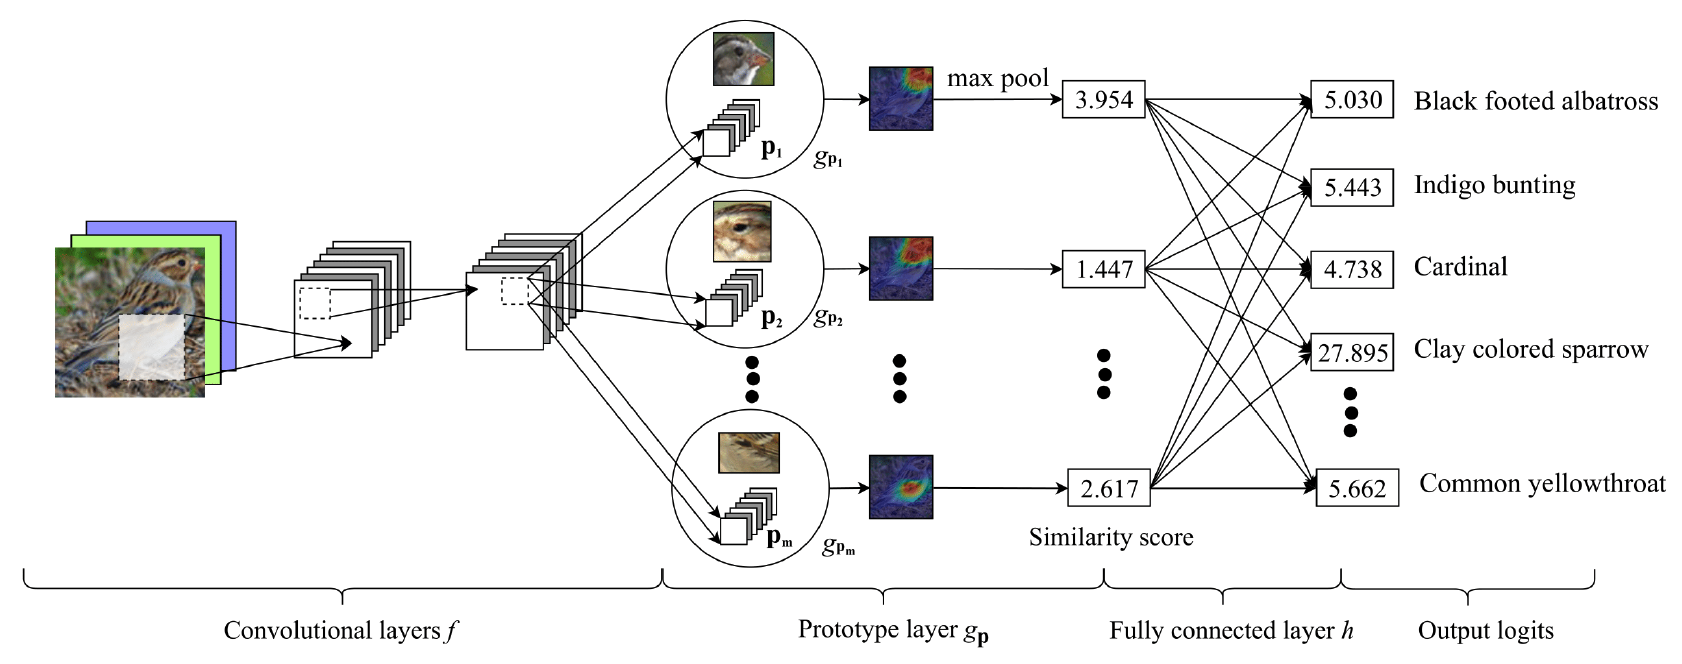
\includegraphics[width=\textwidth]{imgs/ProtoPNet.png}
    \caption{ProtoPNet \citep{chen_this_2019}}
    \label{fig:ProtoPNet}
\end{subfigure}
\hfill
\begin{subfigure}{0.45\textwidth}
    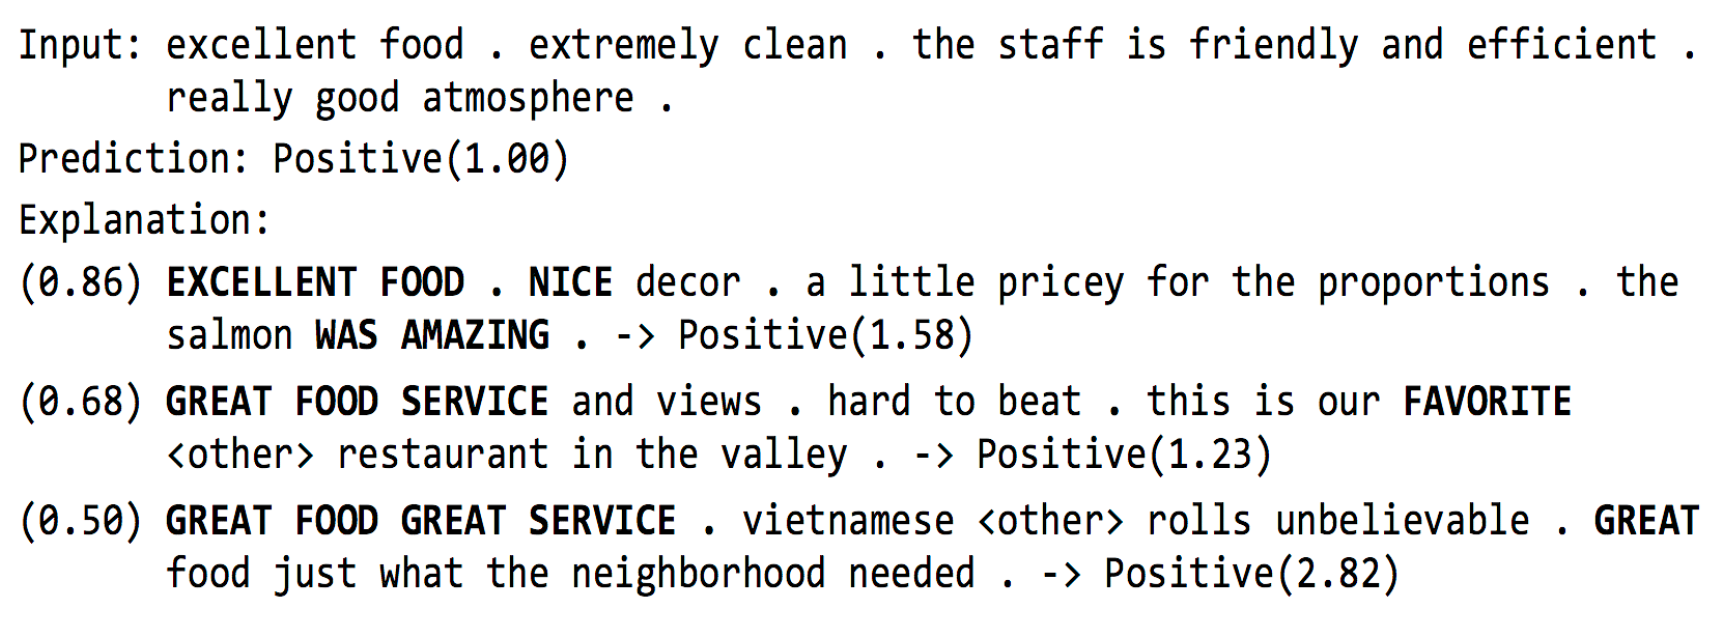
\includegraphics[width=\textwidth]{imgs/ProSeNet.png}
    \caption{ProSeNet Example \citep{ming_interpretable_2019}}
    \label{fig:ProSeNet}
\end{subfigure}
\caption{Existing Prototype Learning Models}
\end{figure}

Prototype learning has been extended to interpret text classification. In this vein, \cite{ming_interpretable_2019} propose ProSeNet, which adds the prototype layer after the sequence encoder (e.g., RNN). This model is able to predict the class of a sentence (e.g., positive or negative) and explain which part of the sentence (prototype) leads to such a prediction result. 
Figure \ref{fig:ProSeNet} shows an example, where the input is classified as positive because it strongly presents positive prototypes, such as ``excellent food'' and ``great food service.''
A number of prototype learning models have also been proposed for various tasks. For example, \cite{rymarczyk_protopshare_2021} develop ProtoPShare that captures sharing property between each pair of prototypes. \cite{nauta_neural_2021} combine decision trees and prototype learning so that the prototype reasoning process can be streamlined as a tree structure. \cite{singh_these_2021} design two groups of prototypes: one group that the input looks like and the other group that the input does not look like. Table \ref{tb:prototypelearning} contrasts major prototype learning methods with our method.

% https://tex.stackexchange.com/questions/211898/putting-several-footnotes-below-the-table
\begin{table}[h]
\centering
\caption{Existing Prototype Learning Methods vs. Our Method}
\label{tb:prototypelearning}
\small
\begin{threeparttable}
\begin{tabular}{lL{85pt}L{140pt}L{75pt}L{15pt}}
\toprule
% \midrule
  Study & Model & Novelty & Input &  TP\tnote{*}\\ \midrule
 \cite{chen_this_2019}& ProtoPNet & Prototype for image classification & An image &  No\\
 \cite{hase_interpretable_2019}& HPNet & Hierarchical prototype & An image &  No\\
 \cite{ming_interpretable_2019}& ProSeNet & Prototype for text classification & A piece of text & No \\
 \cite{xu_attribute_2020}& APN & Represent attribute for zero-shot learning & An image &  No \\
 \cite{shitole_one_2021}& Structured Attention Graphs & Attention maps to explain a classifier & An image & No \Tstrut \\
 \cite{rymarczyk_protopshare_2021}& ProtoPShare & Prototype parts share & An image & No \\
 \cite{nauta_neural_2021}& ProtoTree & Prototype and decision tree & An image & No \\
 \cite{wang_interpretable_2021}& TesNet & Add embedding space using manifold & An image & No \\
 \cite{singh_these_2021}& NP-ProtoPNet & Positive reasoning and negative reasoning & An image & No \\
 \cite{nauta_this_2021}& Explain ProtoPNet & Generate textual info about prototypes & An image & No \\


 Our Method& TempPNet & Capture temporal progression of the input & A sequence of walking tests & 
 % \checkmark
 Yes \\ \bottomrule
\end{tabular}
\begin{tablenotes}\footnotesize
    \item[*] TP stands for ``Temporal Progression'', indicating whether a model is capable of detecting interpretable temporal progression patterns from its input and then leveraging these patterns for prediction and interpretation. We articulate this point in Section \ref{sec:lr:tidl}.
\end{tablenotes}
\end{threeparttable}
\end{table}

\subsection{Key Novelties of Our Study} \label{sec:lr:tidl}

Our literature review reveals several research gaps and opportunities for methodological innovation. Prior health sensing research mostly focuses on chronic disease prediction but generally overlooks depression prediction. Although a few studies attempt to predict depression using mobility and sensor data, they are ML-based and are either black-box models or models that explain predictions based on simple features (e.g., mean and variance) of sensor data, which are undesired for healthcare applications. Different from these studies, our research devises a novel interpretable deep learning model for depression prediction, following the cutting-edge prototype learning paradigm.


Although existing prototype learning methods offer an exciting mode of prediction and interpretation, they fall short in the present study. These methods make predictions and interpretations from a single input (e.g., an image or a sentence) and define their prototypes for individual components of that input (e.g., the head of a clay-colored bird). 
In contrast, our method takes a sequence of inputs because each patient performs a sequence of walking tests. 
The temporal dimension of our method's inputs has practical implications because
medical literature suggests that depression symptoms are progressive and have multiple phases \citep{ bockting_lifetime_2015,dattani_mental_2021}. As depicted in Figure \ref{fig:depression_trend}, from the onset phase, a patient's symptom severity may trend up and progress to acute depression. After the acute phase, some patients' symptoms may peak and flatten, while others could exacerbate. A portion of the patients may recover from depression, and their symptom severity trends down. At any timepoint, a recovered patient is likely to relapse, and symptoms will subsequently recur and their severities may fluctuate. 
\begin{figure}[h]
    \centering
    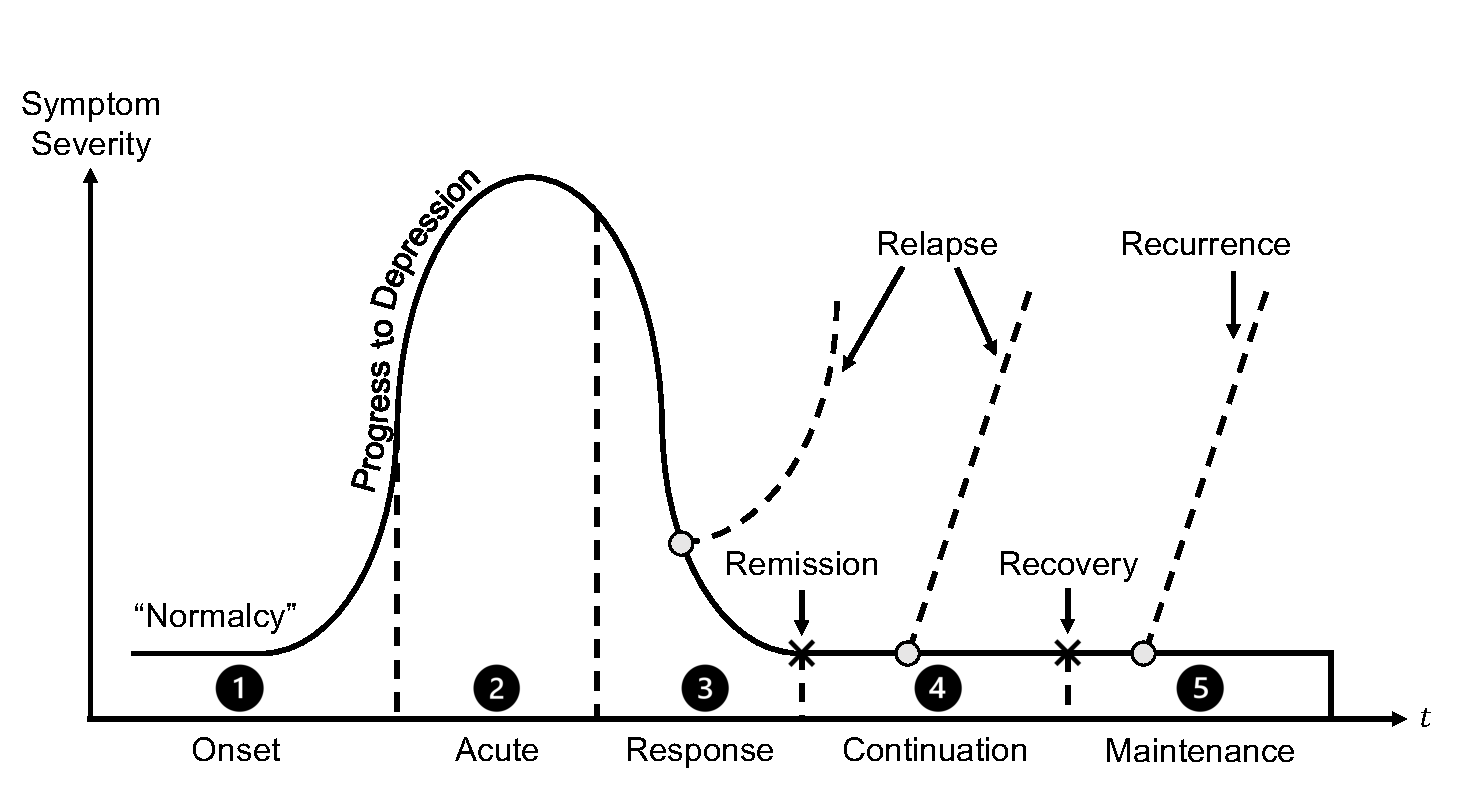
\includegraphics[width=0.6\textwidth]{imgs/depression_trend.pdf}
    \caption{Temporal Progression of Depression \citep{bockting_lifetime_2015}}
    \label{fig:depression_trend}
\end{figure}

When applying existing prototype learning methods to our study, we are able to determine to what extent a single walking test is ``normal''. 
However, no depression symptom in a single walking test does not imply that the patient has no depression because the test might be performed at the ``normalcy phase,'' which could just be transitory and would quickly progress to severe depression. 
As a result, it is essential to predict and interpret the mental state of a patient based on a temporal sequence of walking tests that characterizes the full course of symptom progression. 
Motivated by this fact and the depression progression literature \citep{bockting_lifetime_2015,dattani_mental_2021}, we aim to design a novel prototype learning method that predicts and interprets the occurrence of depression based on prototypical temporal symptom progression detected from walking test sequences.


 


\section{Problem Formulation} \label{sec:problem_formulation}

For a patient $u$, let $y^{(u)}$ be the patient's depression status, where $y^{(u)}=1$ denotes depression, and $y^{(u)}=0$ represents non-depression. 
%The value of $y^{(u)}$ can be obtained through a survey after the patient's walking tests. 
We also observe this patient's $N_u$ walking tests denoted by $X^{(u)}=\langle X^{(u)}_1,X^{(u)}_2,\dots,X^{(u)}_{N_u} \rangle$ that are performed at timepoints $\langle t^{(u)}_1, t^{(u)}_2, \dots, t^{(u)}_{N_u} \rangle$. Each walking test is comprised of three tasks: walking outbound for 30 seconds, returning to the original place, and standing for 30 seconds. The $i$th walking test $X_i^{(u)}$ observed at timepoint $t^{(u)}_i$ (e.g., 2015-05-04) is comprised of a sequence of regularly sampled sensor data: $X^{(u)}_i= \langle a_1, a_2,\dots,a_L \rangle $, where vector $a_l$ is the sensor feature sampled at timepoint $l$ (e.g., $1850$ milliseconds after the start of the walking test).\footnote{In our context, sensor signals are sampled with a fixed frequency. For example, a sampling frequency of 100Hz means that one sensor feature vector is collected per 0.01 second. To simplify notation, we omit the specificity to walking test and patient in notation $a_l$ (a sensor feature) and $L$ (the length of a sensor signal sequence). Note that different sensor signal sequences could have different lengths.} 
Each sensor feature $a_l$ is derived from the accelerometer readings 
and gyroscope readings 
recorded for the three tasks in the walking test. Please see Appendix \ref{apd:sen_features} for the details of $a_l$.

Let $\mathcal{U}$ denote the set of patients. We observe the dataset $\mathcal{D}=\{(X^{(u)},y^{(u)} )|u=1,2,\dots,|\mathcal{U}| \}$, where $X^{(u)}$ and $y^{(u)}$ represent the sequence of walking tests and the depression status of patient $u$, respectively, and $|\mathcal{U}|$ denotes the number of patients. The objective of the problem studied is to learn a model from $\mathcal{D}$ that can predict the depression status of a new patient, based on sensor data collected from the patient's walking tests, and interpret the prediction. Table \ref{tb:notation} summarizes the important notations used in this paper.

To solve this problem, it is critical to learn two kinds of prototypes from $\mathcal{D}$: symptom prototypes (e.g., short strides and slow gait velocity) and trend prototypes (e.g., symptom severity trending up, trending down, and fluctuating). To learn these prototypes, we need to tackle three methodological challenges. First, while rich sensor data can be collected during a walking test, it is non-trivial to define prototypes representing depression symptoms, such that their existing strength\footnote{Existing strength is defined as how strongly a depression symptom presents in a walking test.} in a walking test can be interpreted as the snapshot of symptom severity at the time of the walking test. 
Second, the elapsed time between two consecutive walking tests is irregular. For example, a patient might take the second walking test one day after the first one, while taking the third test four days after the second one. 
On the one hand, it is essential to explicitly consider these irregular inter-test time intervals when inspecting the time series of symptom severities, because they reveal the progression of symptom severities and enable the definition of prototypes representing temporal depression symptom progression.
On the other hand, existing prototype learning methods cannot deal with sequential inputs that are irregularly spaced in time, as indicated by the TP column in Table \ref{tb:prototypelearning}. This gap motivates us to develop a novel and effective method to analyze this new type of input for prototype learning.
Lastly, different patients often conduct varying numbers of walking tests within an observation time window. It is also unknown which phase of depression progression each walking test is performed at. 
Consequently, given a prototypical temporal symptom progression, it is difficult to measure its existing strength in a walking test sequence because the two objects are not aligned in time. That is, for each walking test, we do not know against which part of the prototypical progression the walking test should be compared. 
In the next section, we develop a novel method that explicitly addresses these three challenges.


\begin{table}[h]
\caption{Notation}
\label{tb:notation}
\small
\centering
\begin{threeparttable}
\begin{tabular}{L{0.1\textwidth} L{0.85\textwidth}}
\toprule
Notation &  \multicolumn{1}{c}{Description} \\ \midrule
$X_i$ & The sensor signal sequence of the $i$th walking test of a focal patient. \\
$t_i$ & The timepoint when the walking test $X_i$ is performed. \\
$H_i^{\mathbb{S}}$ & The feature matrix extracted from walking test $X_i$. \\
$p_m^{\mathbb{S}}$ & The embedding vector for symptom prototype $m$. \\
$s_{m,i}^{\mathbb{S}}$ & The existence strength of symptom prototype $m$ in walking test $X_i$, or the severity of symptom $m$ detected in the walking test, defined by Equation \ref{eq:s_m_i}. \\
$S$ & The symptom progression matrix detected for the focal patient, defined by Equation \ref{eq:sym_prog_mat}. \\
$\mathcal{G}^{(k)}(t)$ & The definition of trend prototype $k$, defined by Equation \ref{eq:g_k_t}. \\
% $p_k^{\mathbb{T}}$ & The coefficient matrix specifying trend prototype $k$ \\
$s_k^{\mathbb{T}}$ & The existence strength of trend prototype $k$ in symptom progression matrix $S$, defined by Equation \ref{eq:s_k_trend_final}. \\
\bottomrule
\end{tabular} 
\end{threeparttable}
\end{table}



\section{The TempPNet Approach} \label{sec:method}

To overcome the above-mentioned technical challenges, we present the \underline{Temp}oral \underline{P}rototype \underline{Net}work (TempPNet), an interpretable classifier equipped with a novel temporal prototype layer that predicts depression status based on the prototypical temporal progression of walking symptoms. 
Figure \ref{fig:main_model} shows the architecture of our model, which features three building blocks: a feature extraction layer that represents a sequence of walking tests as a sequence of features, a temporal prototype layer that defines symptom prototypes and trend prototypes for depression detection and then computes the existing strength of these prototypes in a walking test sequence, and lastly a classification layer that classifies a patient into depression or non-depression categories based on the existing strength of trend prototypes.
\begin{figure}[h]
    \centering
    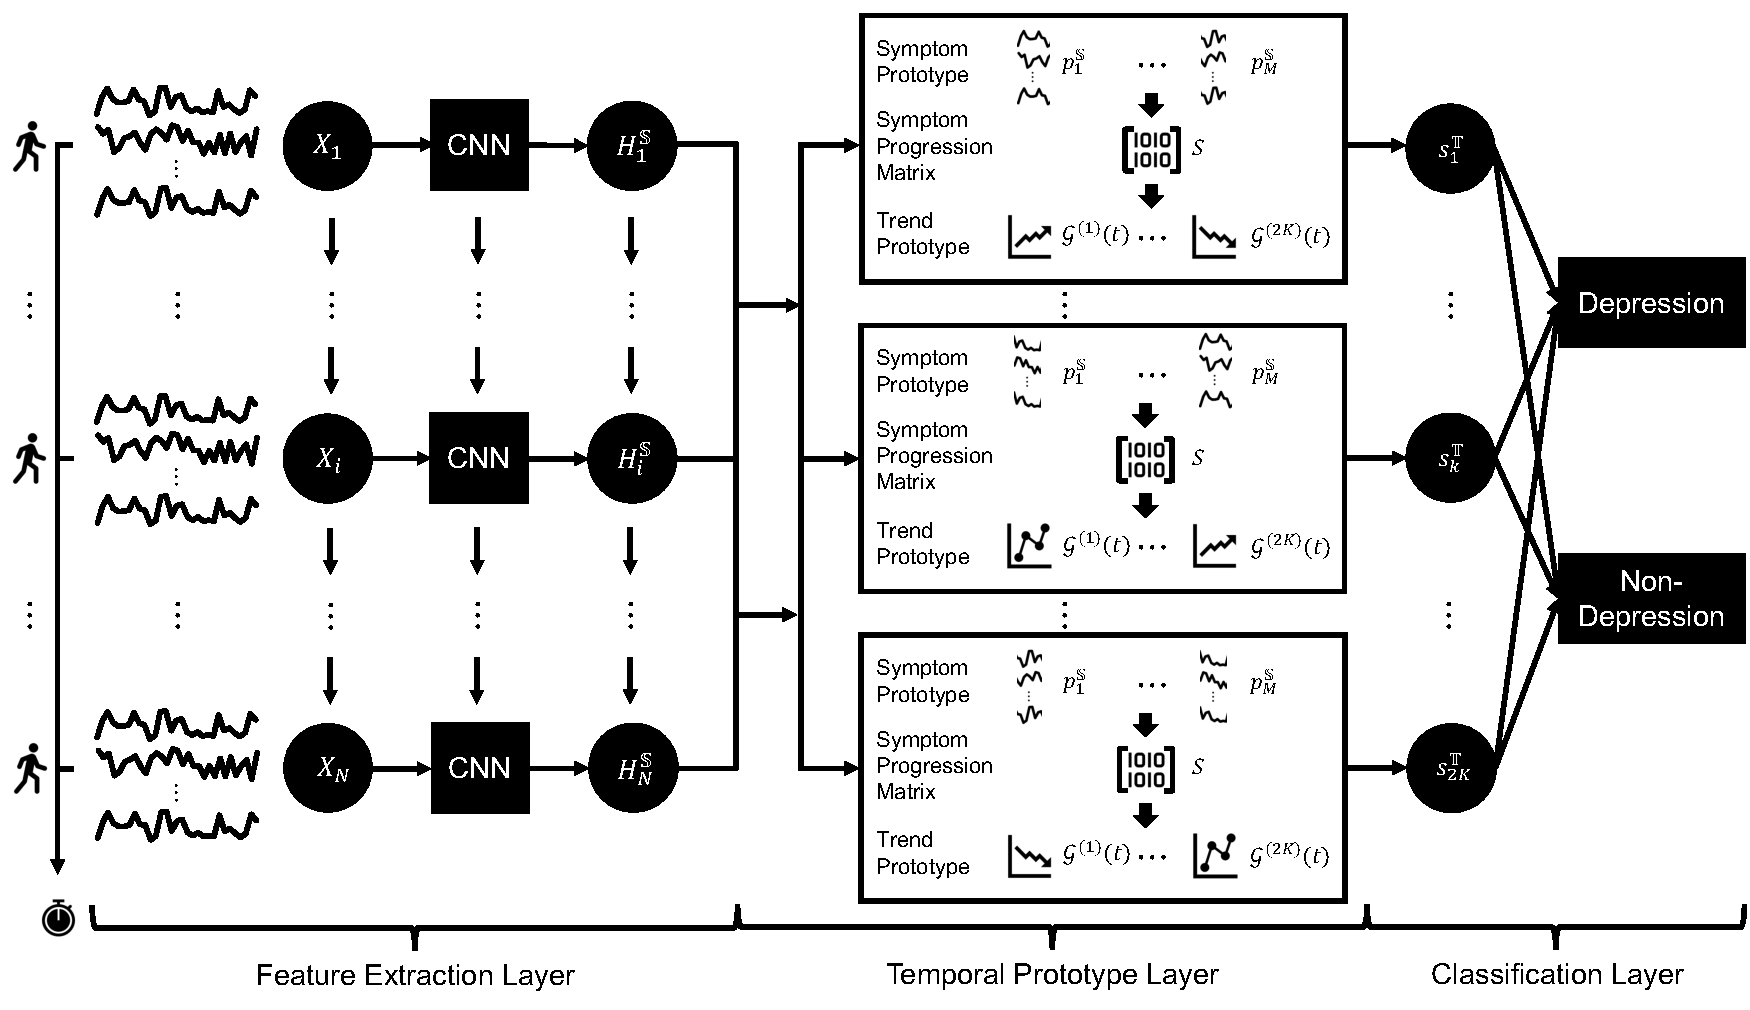
\includegraphics[width=\textwidth]{imgs/main_model.pdf}
    \caption{TempPNet Architecture}
    \label{fig:main_model}
\end{figure}
We organize the method description as follows. 
Section \ref{sec:method:mat} introduces the feature extraction layer and the symptom prototypes, based on which we propose the symptom progression matrix, the foundational artifact of TempPNet. 
Next, we proceed to the design of the trend prototypes in Section \ref{sec:method:trend} for detecting prototypical symptom progression patterns of depression state. 
We then finish the development of TempPNet in Section \ref{sec:method:lr_obj} by specifying the classification layer and the learning objective. 

\subsection{The Symptom Prototype and Symptom Progression Matrix } \label{sec:method:mat}

In the following discussion, we consider a focal patient $u$, and thus drop the superscripts and subscripts related to the patient to simplify the notation. Recall that we can observe a sequence of $N$ walking tests for this patient, whose $i$th walking test is represented by the sensor signal sequence $X_i$. To learn an effective representation of $X_i$, we employ a deep Convolutional Neural Network (CNN) layer \citep{goodfellow_deep_2016, zhang_deep_2020}. Let $H_i^{\mathbb{S}}\in R^{n_o \times n_e}$ denote the learned embedding matrix for the sensor signal sequence $X_i$, where $n_o$ is the number of patches generated by the deep CNN layer and $n_e$ is the embedding dimension of each patch \citep{chen_this_2019}. We define $H_i^{\mathbb{S}}$ as

\begin{equation}
\label{eq:h_i_sym}
H_{i}^{\mathbb{S}} = \text{CNN}(X_{i})
\end{equation}
where the specifications of the deep CNN layer are articulated in Appendix \ref{apd:cnn}. Let $H_{o|i}^{\mathbb{S}}$ denote the $o$th column of $H_{i}^{\mathbb{S}}$. 
The key benefit of using CNN for learning the embedding of $X_i$ is that each patch $H_{o|i}^{\mathbb{S}}$ has its own receptive field,\footnote{A receptive field is the region in which an optimal stimulus elicits vigorous response from a neuron \citep{goodfellow_deep_2016}} which can be identified and visualized as a local segment in $X_i$. Following \cite{chen_this_2019}, we identify the symptoms at the receptive field level.
We articulate how to leverage this property to inspect the learned prototypes in Section \ref{sec:method:proto_viz}.
Equation \ref{eq:h_i_sym} corresponds to the feature extraction layer of TempPNet in Figure \ref{fig:main_model}.

Similar to prototype learning in image recognition, we aim to detect what prototypical walking symptoms $H_{i}^{\mathbb{S}}$ (the representation of $X_i$) resembles. For this purpose, we need to learn $M$ symptom prototypes that represent typical walking symptoms, such as short strides and slow gait velocity \citep{lemke_spatiotemporal_2000, michalak_embodiment_2009, czech_gaitpy_2019}. These symptom prototypes are defined as the latent representation of prototypical waking patterns in the input signal. We embed each symptom prototype $m$ as a vector $p_m^{\mathbb{S}} \in R^{n_e}$ for $m=1,2,\dots,M$, which is in the same latent space as $H_{i}^{\mathbb{S}}$. Following the common strategy of prototype learning \citep{chen_this_2019}, symptom prototype vector $p_m^{\mathbb{S}}$ will be learned as model parameters, and then identified as and visualized by the walking test segment where it presents most strongly. The interpretation mechanism is to find the prototypical patterns within the input sensor signal that are indicative of depression walking symptoms and thereby informative for depression prediction. The middle part of Figure \ref{fig:main_model} provides an exemplar visualization of the symptom prototypes.
Let $s_{m,i}^{\mathbb{S}}$ denote the existing strength of symptom prototype $m$ in walking test $X_i$, which can also be understood as the severity of symptom $m$ detected in the walking test. We define $s_{m,i}^{\mathbb{S}}$ as
\begin{subequations}
\label{eq:s_m_i}
\begin{align}
  s_{o|m,i}^{\mathbb{S}} &= \exp⁡(\gamma -{||H_{o|i}^{\mathbb{S}}-p_m^{\mathbb{S}}||}_2^2) \\
  s_{m,i}^{\mathbb{S}} &= \max_{o=1,2,\dots,n_o} s_{o|m,i}^{\mathbb{S}}
\end{align}
\end{subequations}
where $\gamma < 0$ is an infinitesimal constant to ensure $0 < s_{o|m,i}^{\mathbb{S}} < 1$ for $o=1,2,\dots,n_o$.
A high value of $s_{o|m,i}^{\mathbb{S}}$ suggests that strong existence of symptom prototype $m$, or high severity of walking symptom $m$, is detected in the $o$th region in walking test $X_i$. As a result, $s_{m,i}^{\mathbb{S}}$ measures the overall severity of symptom prototype $m$ in walking test $X_i$. 

Unlike existing prototype learning studies that predict and interpret based on static prototypes solely \citep{chen_this_2019,ming_interpretable_2019}, the severity of symptom prototype $s_{m,i}^{\mathbb{S}}$ is dynamic and forms a temporal progression pattern, as we observe patients' sensor data over time.
By collecting the severity scores of all symptom prototypes across the sequence of walking tests, we can construct the symptom progression matrix $ S \in R^{M \times N}$ as 
\begin{equation}
\label{eq:sym_prog_mat}
S = \begin{blockarray}{ccccc}
 t_1 & t_2 & \dots & t_N & \\
\begin{block}{[cccc]c}
s_{1,1}^{\mathbb{S}} & s_{1,2}^{\mathbb{S}} &\cdots & s_{1,N}^{\mathbb{S}} & \text{sym}_1 \bigstrut[t] \\
s_{2,1}^{\mathbb{S}} & s_{2,2}^{\mathbb{S}} & \cdots & s_{2,N}^{\mathbb{S}} & \text{sym}_2  \\
  \vdots & \vdots & \ddots & \vdots & \\
 s_{M,1}^{\mathbb{S}} & s_{M,2}^{\mathbb{S}} &\cdots & s_{M,N}^{\mathbb{S}} & \text{sym}_M \bigstrut[b]\\
\end{block}
\end{blockarray}
% \vspace*{-1.25\baselineskip}
\end{equation}
where we label each column by the timepoint when the corresponding walking test is performed, and each row by the corresponding symptom prototype ($\text{sym}_m$ denotes symptom $m$).
In matrix $S$, the $m$th row corresponds to the temporal progression of the severities of symptom $m$, while the $i$th column corresponds to the \textit{contemporaneous distribution of symptom severities} observed at timepoint $t_i$. In other words, if we regard each symptom severity as a random variable that randomly evolves over time, then the column vector $S_i$ is a realization of these $M$ random variables drawn from their joint distribution specific to timepoint $t_i$.
From this perspective, the symptom progression matrix describes how the severities of the $M$ symptoms co-evolve over time. 
To make an interpretable prediction, we need to detect whether such a matrix resembles typical depression or non-depression symptom progression trends such as in Figure \ref{fig:depression_trend}, which we define as trend prototypes in this study. In the next section, we introduce the computation of trend prototypes. 


\subsection{Detecting Prototypical Depression Symptom Progression Trends} \label{sec:method:trend}


We first present a conceptual overview of our definition of trend prototype and then discuss the technical details in the subsections.
We aim to learn $2K$ trend prototypes: $K$ for the depression category and the remaining $K$ for the non-depression category. 
We view each trend prototype as a prototypical continuous co-evolution trajectory of the $M$ symptom severities over time, such as trending up, trending down, and fluctuating. Therefore, a trend prototype can be defined as a continuous vector-valued function of time.
Let $\mathcal{G}^{(k)}(t)$ denote the $k$th trend prototype, which maps a time scalar to a vector of symptom severities of length $M$. 
The mathematical details of $\mathcal{G}^{(k)}(t)$ will be given in Section \ref{sec:method:proto_layer:g_k_trend}.
We offer a particular interpretation of trend prototypes: if the focal patient's symptom progression matrix $S$ strongly resembles trend prototype $k$, then the symptom severities $S_i$ detected at timepoint $t_i$ should be close to $\mathcal{G}^{(k)}(t_i)$.\footnote{We use the word ``close'' rather than ``identical'' for the definition of trend prototype because the symptom progression matrix of a particular patient is likely to exhibit some idiosyncratic progression patterns that are not common enough to be regarded as prototypical, and therefore $S_i$ is likely to randomly deviate from $\mathcal{G}^{(k)}(t_i)$ by a small amount.} Based on this interpretation, the existing strength of trend prototype $k$ in symptom progression matrix $S$ can be measured as the overall closeness between $S_i$ and $\mathcal{G}^{(k)}(t_i)$ over observation timepoints $\langle t_1, t_2, \dots, t_{N} \rangle$. The implementation of this is articulated in Section \ref{sec:method:proto_layer:s_k_trend}.


\subsubsection{The Definition of Trend Prototypes:} \label{sec:method:proto_layer:g_k_trend}

A trend prototype is a continuous function of time that characterizes the evolution of symptom severities. This goal necessitates a continuous function that can trace any freely-valued trajectory over time. Studies have shown that any trajectory over time can be decomposed into a summation of sine and cosine curves in the frequency domain \citep{xu_inductive_2020, wang_word2fun_2021}. Inspired by those works, we design the trend prototype as follows. Let $\mathcal{G}_{m}^{(k)}(t)$ denote the severity of symptom $m$ at timepoint $t$ given by trend prototype $k$. Leveraging the time encoding method in \cite{xu_inductive_2020}, we compute $\mathcal{G}_{m}^{(k)}(t)$ as 
\begin{equation}
\label{eq:g_m_k}
\begin{aligned}
\mathcal{G}_{m}^{(k)}(t) &= \sigma \Big( \sqrt{\frac{1}{n_d}} \sum_{j=1}^{n_d} p_{k,m,j}^{\mathbb{T}} \cos(\omega_j t + \theta_j) + \sqrt{\frac{1}{n_d}} \sum_{j=1}^{n_d} p_{k,m,n_d+j}^{\mathbb{T}} \sin(\omega_j t + \theta_j) \Big) \\
  &= \sigma \big( \Phi ( t )^T p_{k,m}^{\mathbb{T}} \big)
\end{aligned}    
\end{equation}
where $p_{k,m}^{\mathbb{T}} = [p_{k,m,1}^{\mathbb{T}}, p_{k,m,2}^{\mathbb{T}}, \dots, p_{k,m,2 n_d}^{\mathbb{T}} ]^T \in R^{2 n_d}$ is the coefficient vector specific to trend prototype $k$ and symptom prototype $m$, $\Phi(t)$ is the time encoding function \citep{xu_inductive_2020} that transforms timepoint $t$ from a scalar to a numeric vector, defined as
\begin{equation}
\label{eq:time_encoding}
\begin{aligned}
\Phi(t) = \sqrt{\frac{1}{n_d}} \big[ &\cos(\omega_1 t+\theta_1), \cos(\omega_2 t+\theta_2), \dots, \cos(\omega_{n_d} t+\theta_{n_d}), \\
& \sin(\omega_1 t+\theta_1), \sin(\omega_2 t+\theta_2), \dots, \sin(\omega_{n_d} t+\theta_{n_d}) \big]^T
\end{aligned}
\end{equation}  
which is parameterized by frequency vector $\omega=[\omega_1,\omega_2,\dots,\omega_{n_d}]$ as well as phase vector $\theta=[\theta_1,\theta_2,\dots,\theta_{n_d}]$, and lastly $\sigma(.)$ is the sigmoid function defined as $\sigma(x)=1/\big(1+\exp(-x)\big)$ to ensure $0 < \mathcal{G}_{m}^{(k)}(t) < 1$ such that $\mathcal{G}_{m}^{(k)}(t)$ and $s_{m,i}^{\mathbb{S}}$ are in the same range and therefore comparable to each other.
Let $\sigma^{-1}(.)$ denote the inverse of the sigmoid function. Namely, $\sigma^{-1}(x)=\log \frac{x}{1-x}$. 

Our design of $\Phi(t)$ ensures that $\sigma^{-1}\big( \mathcal{G}_{m}^{(k)}(t) \big)$ is able to trace a freely-valued trajectory over time so that the trajectory of symptom severities can be seamlessly modeled by a continuous function. 
By learning the three vectors $p_{k,m}^{\mathbb{T}}$, $\omega$ and $\theta $ as model parameters, while treating $n_d$ as a hyperparameter, Equation \ref{eq:g_m_k} amounts to learning a prototypical temporal progression of symptom $m$ in the frequency domain. In a compact form, trend prototype $k$ can be written as
\begin{equation}
\label{eq:g_k_t}
\mathcal{G}^{(k)}(t) = \sigma \big( p_k^{\mathbb{T}} \Phi(t) \big)
\end{equation}
where $p_k^{\mathbb{T}} \in R^{M \times 2 n_d}$ is the coefficient matrix that specifies the function representation of trend prototype $k$, and is obtained by row stacking the transpose of vectors $p_{k,m}^{\mathbb{T}}$ for $m=1,2,\dots,M$. We can view $p_k^{\mathbb{T}}$ as the embedding form of trend prototype $k$ that is analogous to $p_m^{\mathbb{S}}$, the embedding form of symptom prototype $m$.

Figure \ref{fig:trend_prototype} shows a few examples of potential depression and non-depression trend prototypes. The depression trend prototypes could be characterized by a rising symptom severity (upper left). Such a severity may have deviations from time to time while keeping the upward trend (upper right). These trend prototypes correspond to the onset and acute phases in Figure \ref{fig:depression_trend}. The non-depression trend prototype may be characterized by a downward severity trend (lower left), suggesting a previously depressed patient is recovering. The non-depression trend prototype could also be a curve fluctuating around a fixed level (lower right), indicating the patient never had depression symptoms or has fully recovered from prior depression. 
When a non-depressed patient relapses, depression trend prototypes, such as the upper two, could reappear in his or her walking sensor data.

\begin{figure}[h]
    \centering
    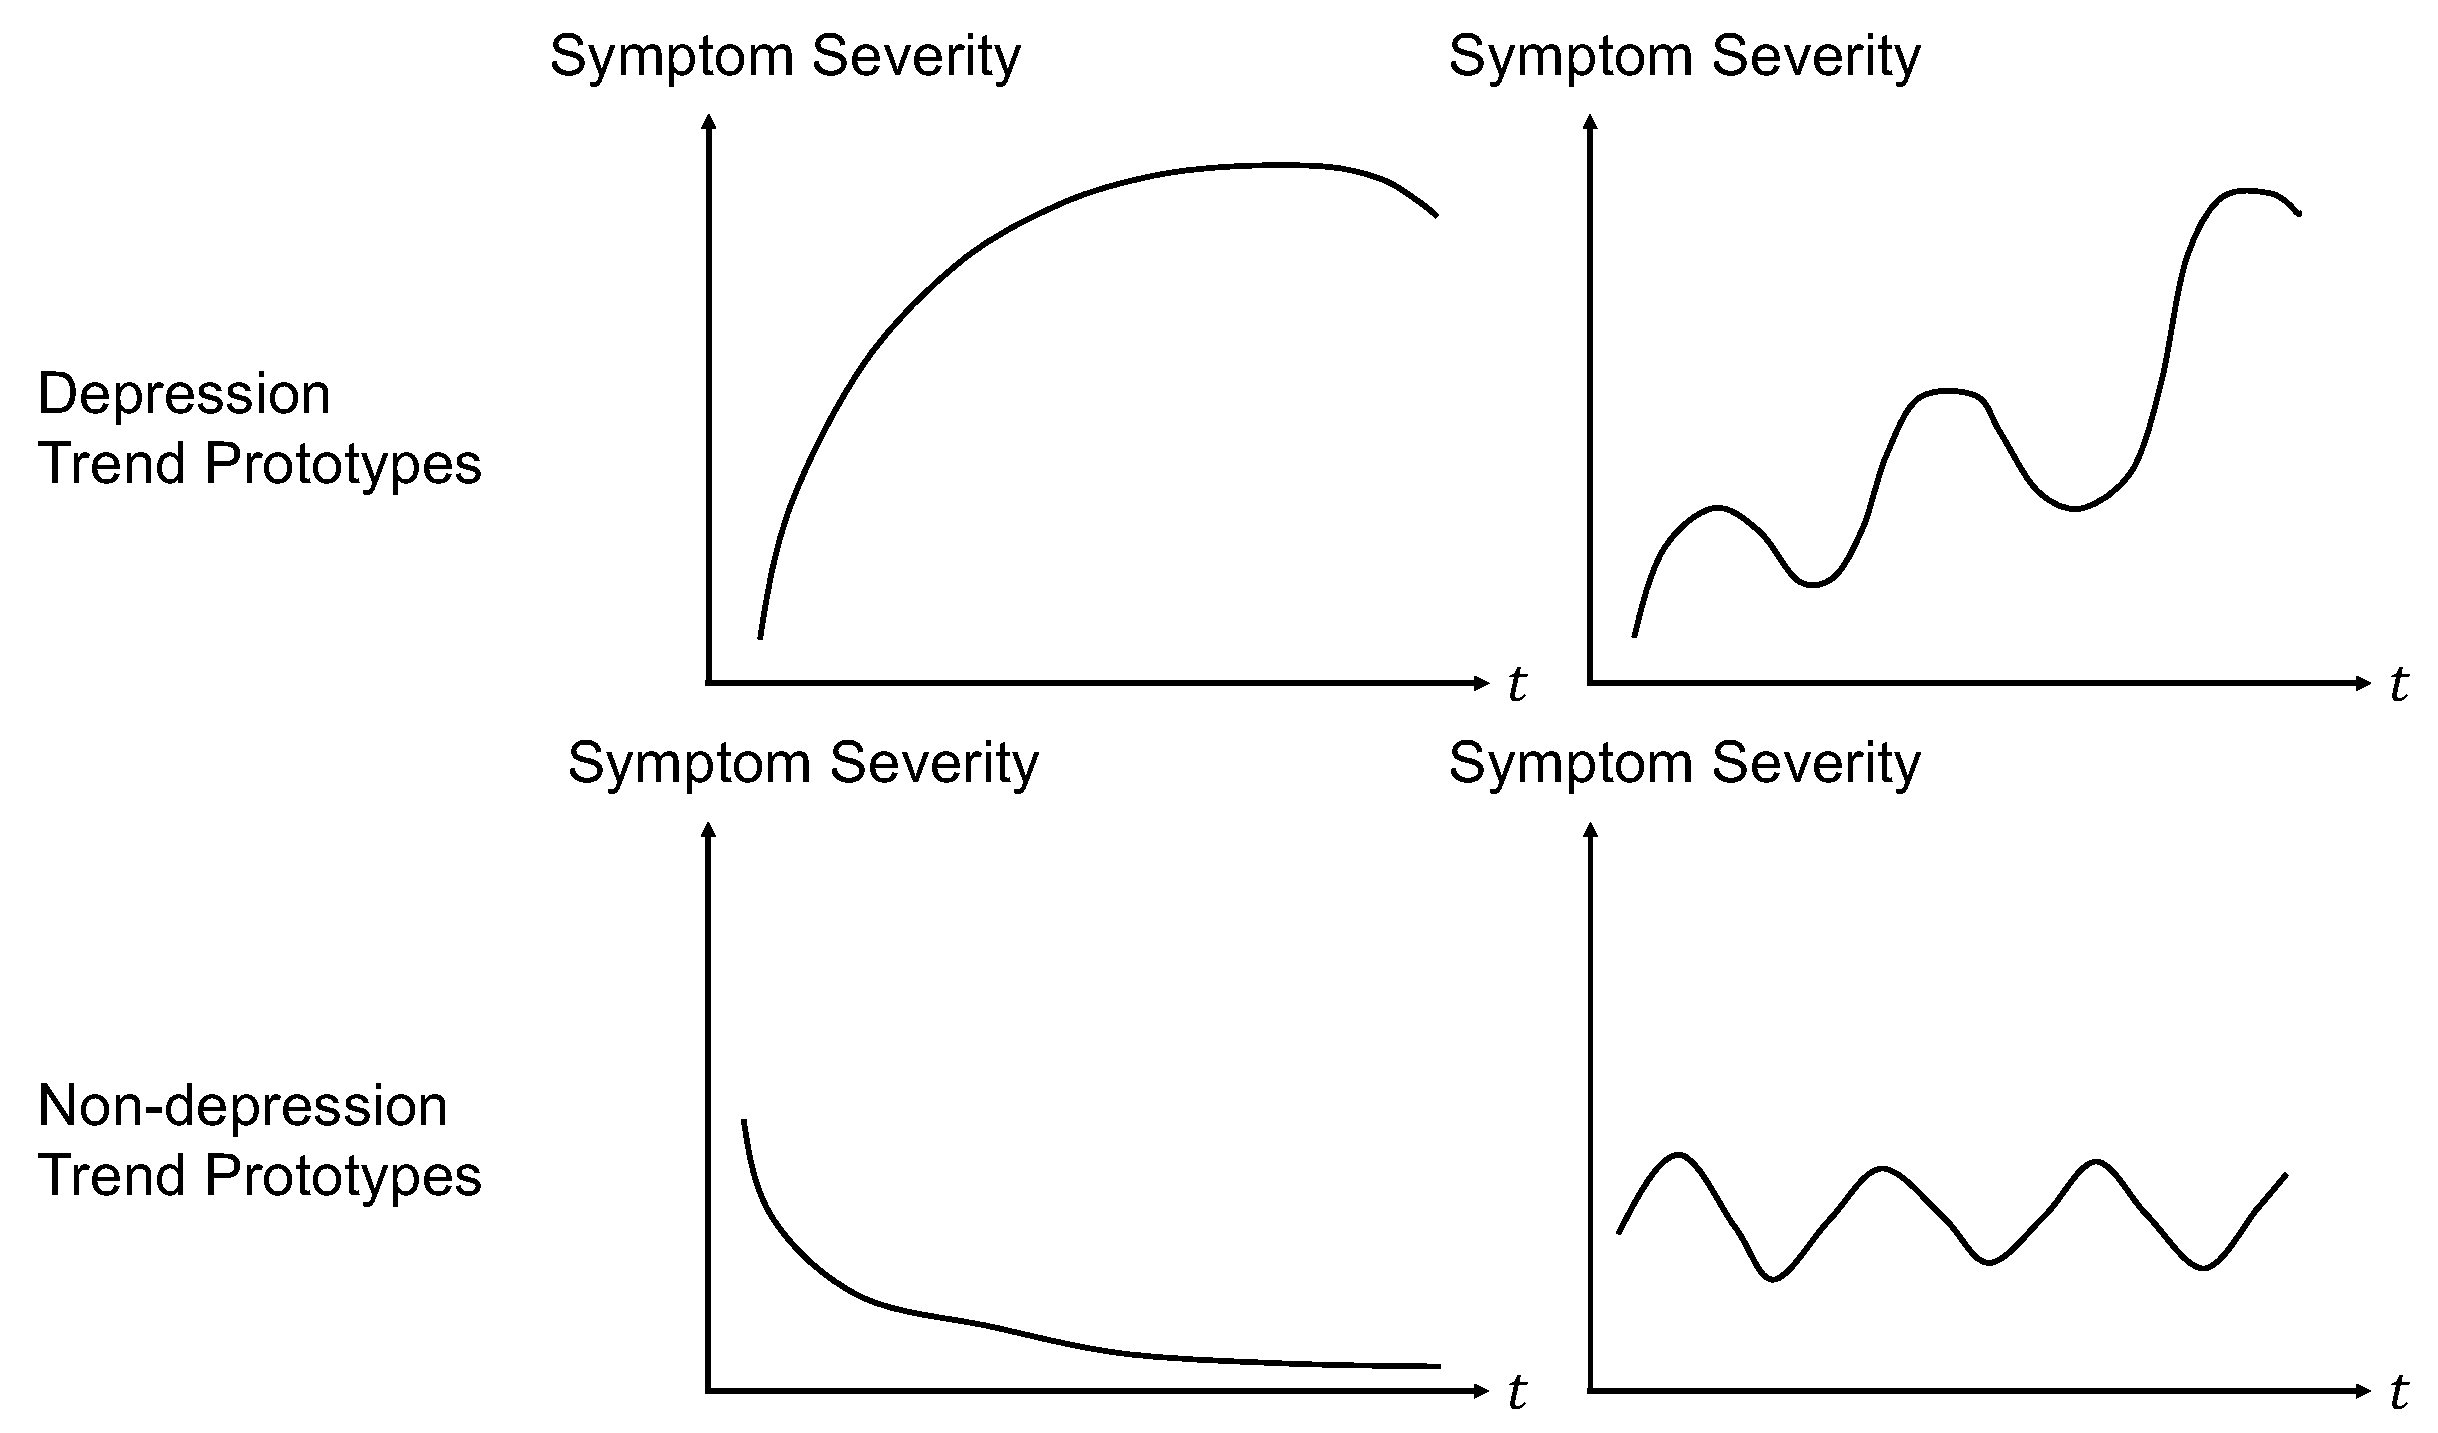
\includegraphics[width=0.7\textwidth]{imgs/trend_prototype.pdf}
    \caption{Examples of Trend Prototype}
    \label{fig:trend_prototype}
\end{figure}

In the subsequent discussion, we will frequently use $\sigma^{-1}\big(\mathcal{G}^{(k)}(t)\big)$, which means applying the inverse of the sigmoid function element-wisely on $\mathcal{G}^{(k)}(t)$. Therefore, we formally define 
\begin{equation}
\label{eq:g_k_t_tilde}
{\tilde{\mathcal{G}}}^{(k)}(t) = \sigma^{-1}\big(\mathcal{G}^{(k)}(t)\big) = p_k^{\mathbb{T}} \Phi(t)
\end{equation}
to simplify the notation.
 

\subsubsection{Detecting the Existing Strength of a Trend Prototype: }\label{sec:method:proto_layer:s_k_trend} 

Let $s_k^{\mathbb{T}}$ denote the existing strength of trend prototype $k$ in symptom progression matrix $S$.
Intuitively, $s_k^{\mathbb{T}}$ should be derived by comparing $S_i$ and $\mathcal{G}^{(k)}(t_i)$ for each timepoint $t_i$, where the former is the ``observed'' symptom severities detected at $t_i$, the latter is its corresponding ``ideal'' values in the prototypical progression patterns captured by trend prototype $k$. The larger the former deviates from the latter across time, the less likely trend prototype $k$ exists in the symptom progression matrix.
However, we argue that for interpretability concerns, $S_i$ should be compared to $\mathcal{G}^{(k)}(t_i-t_0^{(k)})$ rather than $\mathcal{G}^{(k)}(t_i)$, where $t_0^{(k)}$ is a latent variable indicating when the trend starts in the patient's timeline. The computation and rationale of $t_0^{(k)}$ are articulated below.

Recall that Equation \ref{eq:g_m_k} defines $\mathcal{G}^{(k)}(t)$ as a function on the domain $t \in (-\infty, +\infty)$. However, to understand what temporal progression trend prototype $k$ captures, it is necessary to ensure that only a finite segment of $\mathcal{G}^{(k)}(t)$ carries useful information, so that only this segment needs to be visualized to inspect trend prototype $k$. For this purpose, we need to ``bound'' the trend by a starting time and an ending time.
We treat $t=0$ as the starting time of trend prototype $k$, and only work with the right part of $\mathcal{G}^{(k)}(t)$ defined on the non-negative domain $t \in [0, +\infty)$, as shown in Figure \ref{fig:trend_patient}. This design has two implications. Continuing with the example in Figure \ref{fig:trend_patient}, on one hand, $\mathcal{G}^{(k)}(0)$ should be treated as the initial state of trend prototype $k$, and it is the relative timepoint measuring how much time has elapsed since $t=0$ that truly matters. On the other hand, we can only observe the absolute timepoints when the focal patient performs walking tests in reality (e.g., $t_1$, $t_2$, and $t_3$). In general, we cannot assume that $t_1$, the absolute timepoint of the first walking test performed by the patient, is the starting time of trend prototype $k$ in the patient's timeline, because $t_1$ is determined by when the first walking test is performed as well as the range of the observation window. However, the depression progression trend of a patient $\mathcal{G}^{(k)}(t)$ would start regardless of whether a walking test is performed or not. That unobserved trend starting time is noted as $t_0^{(k)}$.
If we were able to observe the zero-th walking test $X_0$ at absolute timepoint $t_0^{(k)}$, and detect symptom severities $S_0$ from it by computing $s_{m,0}^{\mathbb{S}}$ in accordance with Equation \ref{eq:s_m_i} for $m=1,2,\dots,M$, then $S_0$ should be compared to $\mathcal{G}^{(k)}(0)$. 
In this sense, $S_i$, the symptom severity vector detected at $t_i$ in the patient's timeline, should be compared to $\mathcal{G}^{(k)}(t_i-t_0^{(k)})$, the corresponding prototypical values in the trend's timeline.
In Figure \ref{fig:trend_patient}, the detected symptom severity is compared with trend prototype $k$ by aligning the two timelines at a latent personalized trend starting time $t_0^{(k)}$. 

\begin{figure}[h]
    \centering
    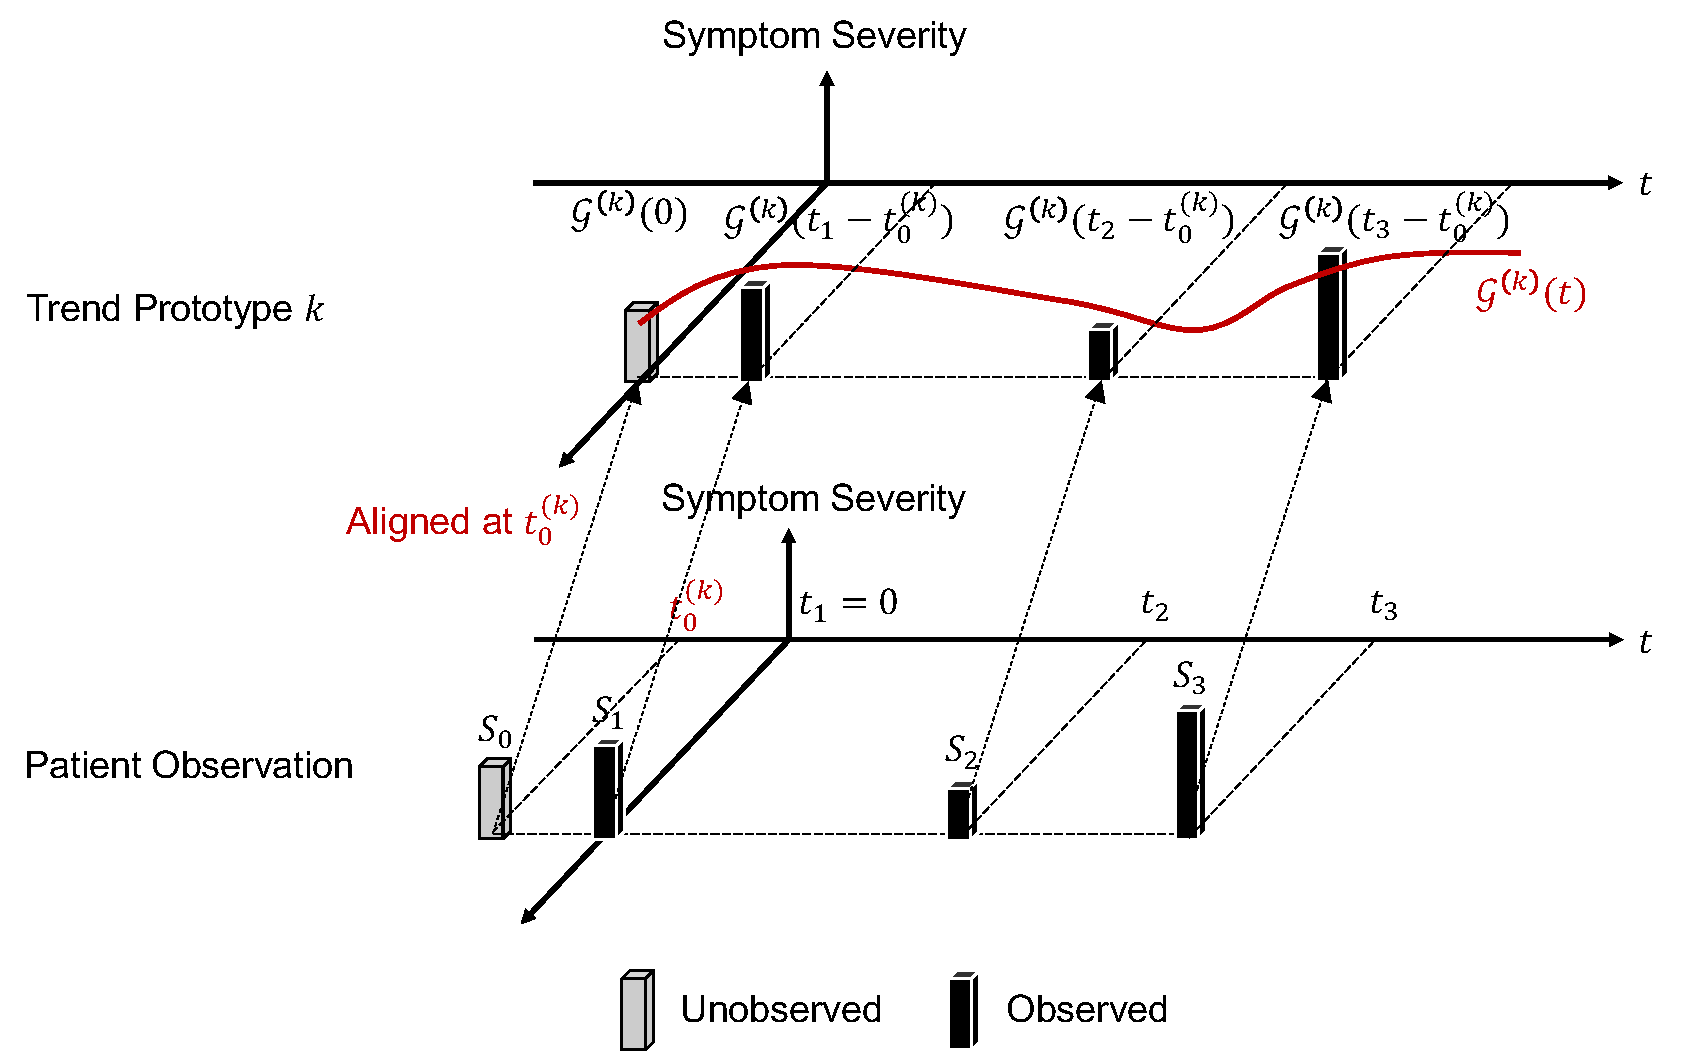
\includegraphics[width=0.7\textwidth]{imgs/trend_patient.pdf}
    \caption{Latent Trend Starting Time}
    \label{fig:trend_patient}
\end{figure}

With $t_0^{(k)}$ at hand, only relative timepoints given by $t_i-t_0^{(k)}$ for $i=1,2,\dots,N$ carry information. As a result, we set $t_1=0$ and measure other timepoints including $t_0^{(k)}$ relative to $t_1$ without loss of generality.
To facilitate the learning of interpretable trend prototypes, we additionally impose the constraint $t_0^{(k)} < t_1=0$. If $t_0^{(k)} > 0$, the symptom severities detected before $t_0^{(k)}$ need to be compared to the left part of $\mathcal{G}^{(k)}(t)$ defined on domain $t \in (-\infty, 0)$, which we intend to avoid for interpretability concerns. 
For example, it is undesired to compare $S_1$ with $\mathcal{G}^{(k)}(t_1-t_0^{(k)})=\mathcal{G}^{(k)}(-t_0^{(k)})$.
Allowing such a comparison is in conflict with our interpretation of $t=0$ as the starting time of trend prototype $k$. Moreover, it also renders the learned function $\mathcal{G}^{(k)}(t)$ hard to inspect, because the progression patterns within the interval $t\in(-t_0^{(k)}, 0)$ also encode some prototypical patterns summarized from data. Given that $t_0^{(k)}$ varies across patients, the meaningful part of $\mathcal{G}^{(k)}(t)$ is different for different patients. 
In contrast, if we enforce $t_0^{(k)}<0$, all detected symptom severities will be compared to the right part of $\mathcal{G}^{(k)}(t)$ defined on the domain $t \in (0, +\infty)$, making $t=0$ a natural patient-independent starting point to inspect $\mathcal{G}^{(k)}(t)$.
Armed with the notion of $t_0^{(k)}$, we proceed to the definition of $s_k^{\mathbb{T}}$ by assuming a pre-computed $t_0^{(k)}$, and then discuss how to infer $t_0^{(k)}$ by the end of this section, where we introduce another design to impose an effective trend ending time. 

As pointed out by \cite{chen_this_2019}, a prototype can be viewed as a cluster, and its existing strength in an instance is essentially a closeness measurement between the instance and the cluster. 
To develop a principled definition of $s_k^{\mathbb{T}}$, we draw inspiration from the Gaussian Mixture Model \citep{murphy_probabilistic_2022}, a classic clustering algorithm, which measures the closeness between an instance and a cluster in terms of how likely the instance can be generated by the Gaussian component characterized by the cluster. By making an analogy in our context, we view the columns of $S$ as being generated from a time-varying distribution characterized by trend prototype $k$ at aligned timepoints $t_i-t_0^{(k)}$ for $i=1,2,\dots,N$. Different from the Gaussian Mixture Model which deals with instances described by freely-valued vectors, the entries of $S$ are bounded in the interval $(0,1)$. To properly specify the generation of the columns of $S$, we leverage the logistic-normal distribution, whose samples fall between $(0,1)$. We introduce this distribution first.

Let $x \sim \mathcal{N}(\mu, \Sigma)$ denote a random vector drawn from the $M$-dimensional normal distribution of mean $\mu \in R^{M}$ and covariance $\Sigma \in R^{M \times M}$.
Let $z=\sigma(x)$, which is obtained by transforming $x$ element-wisely with the sigmoid function such that $0 < z_m=\sigma(x_m) < 1$ for $m=1,2,\dots,M$. Then, $z$ follows $\mathcal{L}\mathcal{N}(\mu, \Sigma)$, the $M$-dimensional logistic-normal distribution with mean $\mu$ and covariance $\Sigma$, and its density can be computed as
\begin{equation}
\label{eq:sigmoid_gauss_density}
\mathcal{L}\mathcal{N}(z|\mu, \Sigma) =
\frac{1}{\prod_{m=1}^{M} z_{m}(1-z_{m})}
\frac{\exp \big( -\frac{1}{2} ( \sigma^{-1}(z) - \mu )^{T}{\Sigma }^{-1} (\sigma^{-1}(z) - \mu) \big) }{\sqrt{(2\pi)^{M} \det [ \Sigma] }}
\end{equation}
where $\sigma^{-1}(z)$ means applying the inverse of the sigmoid function element-wisely on $z$, and $\det[\Sigma]$ is the determinant of matrix $\Sigma$. The derivation of Equation \ref{eq:sigmoid_gauss_density} can be found in Appendix \ref{apd:der_logistic_normal}.


Now, consider a focal patient whose symptom progression matrix exhibits the presence of trend prototype $k$ to some extent. 
In this case, we regard $S_i$ as a realization drawn from the contemporaneous distribution of symptom severities given by $\mathcal{L}\mathcal{N}({\tilde{\mathcal{G}}}^{(k)}(t_i-t_0^{(k)}), I)$, the $M$-dimensional logistic-normal distribution characterized by mean ${\tilde{\mathcal{G}}}^{(k)}(t_i-t_0^{(k)})$ and covariance $I$ (the identity matrix), where ${\tilde{\mathcal{G}}}^{(k)}(t)$ is defined by Equation \ref{eq:g_k_t_tilde}, and $t_0^{(k)}$ is the personalized trend starting time explained previously. 
In our setting, $S_i$ is compared to $\mathcal{G}^{(k)}(t_i-t_0^{(k)})$ at the aligned timepoint $t_i-t_0^{(k)}$, while ${\tilde{\mathcal{G}}}^{(k)}(t)$ depicts the mean series of a time-varying logistic-normal distribution which characterizes some prototypical symptom progression patterns subject to a sigmoid transformation. 
We assume that the covariance of this time-varying distribution is the constant identity matrix for parsimonious concerns. 

The generative process of the symptom progression matrix is summarized in Algorithm \ref{alg:gen_enrich}.
\begin{algorithm}[h]
% \small
\caption{The Generative Process of $S$ Characterized by Trend Prototype $k$}\label{alg:gen_enrich}
\begin{algorithmic}[1]
\State Compute $t_0^{(k)}$ via Equation \ref{eq:infer_t0}.
\State Compute $t_i^{(k)} = t_i - t_0^{(k)}$ for $i=1,2,\dots,N$.
\State Compute ${\tilde{\mathcal{G}}}^{(k)}(t_i^{(k)})$ for $i=1,2,\dots,N$ using Equation \ref{eq:g_k_t_tilde}.
\State Draw $S_{i} \sim \mathcal{L} \mathcal{N}({\tilde{\mathcal{G}}}^{(k)}(t_i^{(k)}), I)$ for $i=1,2,\dots,N$.
\end{algorithmic}
\end{algorithm}
Then, we define $s_k^{\mathbb{T}}$ as a scalar proportional to the log-likelihood of generating the column vectors of $S$ in accordance with Algorithm \ref{alg:gen_enrich}. Specifically,
\begin{equation}
\label{eq:s_k_trend_final}
\begin{aligned}
s_k^{\mathbb{T}} &= \sigma \Big( \log \prod_{i=1}^{N} \mathcal{L}\mathcal{N} \big( S_{i}| \tilde{\mathcal{G}}^{(k)}(t_i^{(k)}), I \big) \Big) \\
&= \sigma \Big( \sum_{i=1}^{N} \sum_{m=1}^{M} \log \frac{1}{S_{m,i}(1-S_{m,i})} - \frac{NM}{2} \log 2\pi  - \frac{1}{2} \sum_{i=1}^{N} || \sigma^{-1}(S_{i})-\tilde{\mathcal{G}}^{(k)}(t_i^{(k)}) ||_2^2   \Big)
\end{aligned}
\end{equation}
where $S_{m,i}$ is the entry at row $m$ and column $i$ in matrix $S$. The second step of Equation \ref{eq:s_k_trend_final} is derived by expanding $\mathcal{L}\mathcal{N} \big( S_{i}| \tilde{\mathcal{G}}^{(k)}(t_i^{(k)}), I \big)$ using Equation \ref{eq:sigmoid_gauss_density} and then simplifying the resulting terms. The intuition is that the more likely the columns of $S$ can be observed from the generative process characterized by $\mathcal{G}^{(k)}(t)$, the stronger the evidence is that trend prototype $k$ exists in the symptom progression matrix of the focal patient. 
Equation \ref{eq:s_k_trend_final} ensures $0< s_k^{\mathbb{T}} < 1$, which means that the existence strength of trend prototypes has the same value range with symptom prototypes as defined by Equation \ref{eq:s_m_i}. Indeed, by comparing Equations \ref{eq:s_k_trend_final} and \ref{eq:s_m_i}, an obvious analogy can be established between the definition of $s_k^{\mathbb{T}}$ and $s_{o|m,i}^{\mathbb{S}}$.


Lastly, we complete the definition of $s_k^{\mathbb{T}}$ by specifying the inference procedure of $t_0^{(k)}$. Because $t_0^{(k)}$ is used to generate the symptom progression matrix $S$, given $S$, we should be able to inversely infer $t_0^{(k)}$. 
Based on this intuition, we introduce an inference network, that takes $S$ and the observation timepoints $\langle t_1, t_2, \dots, t_{N} \rangle$ as input, and outputs $t_0^{(k)}$ as a negative scalar. Specifically, the inference network is defined as
\begin{subequations}
\label{eq:infer_t0}
\begin{align}
h_{i}^{\mathbb{T}} &= \text{GRU}\big(h_{i-1}^{\mathbb{T}}, S_{i} \oplus \Phi(t_i) \big) \label{eq:infer_t0_a} \\
t_0^{(k)} &= - n_w \sigma( w_{k}^T h_N^{\mathbb{T}} ) \label{eq:infer_t0_b}
\end{align}
\end{subequations}
In Equation \ref{eq:infer_t0_a}, $\oplus$ is the concatenation operator, $\Phi(.)$ is the time encoding function defined by Equation \ref{eq:time_encoding} but parameterized separately, GRU is a Gated Recurrent Unit layer \citep{cho_properties_2014} used to capture the temporal information in the symptom progression matrix augmented by time features, and lastly $h_i^{\mathbb{T}} \in R^{n_e}$ is the hidden state of the GRU layer at step $i$. In Equation \ref{eq:infer_t0_b}, $h_N^{\mathbb{T}}$ is the last hidden state of the GRU layer, which serves as a feature vector summarizing the information contained in $S$ and $\langle t_1, t_2, \dots, t_{N} \rangle$, $w_{k} \in R^{n_e}$ is a learnable parameter specific to trend prototype $k$, and $n_w>0$ is a hyperparameter. 
Equation \ref{eq:infer_t0} enforces that $-n_w < t_0^{(k)} < 0$. We impose this constraint to make the learned trend prototype easier to interpret. Consider the case where the observation window is 2 weeks, which means that the time difference between the first and the last walking test is at most 2 weeks. If we set $n_w=1$ (time is measured in weeks), then $t_0^{(k)}$ is at most 1 week before the first walking test, which implies that the symptom severities detected from the last walking test will be compared to $\mathcal{G}^{(k)}(3)$ in the most extreme scenario. Consequently, we only need to inspect the segment of $\mathcal{G}^{k}(t)$ defined on the interval $t \in [0, 3]$, since only this segment has been compared to some real data. In this sense, $n_w$ reflects our belief on which segment of $\mathcal{G}^{k}(t)$ can be learned from data with reasonable qualities. For example, it should be hard to believe that we could learn a high-quality trend prototype spanning 7 weeks from an observation window lasting only 2 weeks.

\subsubsection{Superior Properties of the Trend Prototype:}\label{sec:method:proto_layer:summary} 
First, no matter how irregularly the focal patient has performed walking tests over time, the symptom progression matrix detected from these walking tests can always be compared to each trend prototype in a consistent manner. The irregularity of inter-test time intervals is explicitly considered, because each trend prototype is a continuous function of time, and therefore the differences in inter-test time intervals are reflected in the evaluation differences of function values.
Second, while trend prototype $k$ is learned from irregularly spaced point observations of symptom severities, it can be inspected as a complete temporal symptom progression by evaluating $\mathcal{G}^{(k)}(t)$ at regularly and densely spaced timepoints. Moreover, a trend prototype does not need to be attached to a single patient. Instead, walking test sequences gathered for different patients could be used to learn different segments of a trend prototype, which together pinpoint a complete temporal symptom progression spanning the entire observation window.


\subsection{Learning Objective} \label{sec:method:lr_obj}

The classification layer of TempPNet computes the probability of depression given the input sensor signal $X$ of a focal patient, which is defined as
\begin{equation}
\label{eq:class_layer}
    P(y=1|X) = \sigma \Big( \sum_{k \in \mathcal{K}^{+} } s_k^{\mathbb{T}} - \sum_{k \in \mathcal{K}^{-} } s_k^{\mathbb{T}} \Big)
\end{equation}
where $\mathcal{K}^{+}=\{1,2,\dots,K\}$, $\mathcal{K}^{-}=\{K+1,K+2,\dots,2K\}$, and $s_k^{\mathbb{T}}$ is defined by Equation \ref{eq:s_k_trend_final}. The above definition imposes the relationship that a high probability of depression is due to the detection of strong overall existing strength of depression trend prototypes, while weak overall existing strength of non-depression trend prototypes. 


The objective function of TempPNet to be minimized is defined based on the binary cross-entropy loss with two additional regularization terms. Specifically, 
\begin{equation}
  \label{eq:objective}
   \mathcal{L}_{\text{TempPNet}} = - \frac{1}{|\mathcal{U}|} \sum_{u \in \mathcal{U} } \log P(y^{(u)}|X^{(u)}) + \lambda_{\mathbb{S}} R_{\mathbb{S}} + \lambda_{\mathbb{T}} R_{\mathbb{T}}
\end{equation}
where $P(y^{(u)}|X^{(u)})$ is computed in accordance with Equation \ref{eq:class_layer} for patient $u$, $R_{\mathbb{S}}$ and $R_{\mathbb{T}}$ respectively denote the regularization term for the symptom prototypes and the trend prototypes, and lastly, $\lambda_{\mathbb{S}}$ and $\lambda_{\mathbb{T}}$ are the hyperparameters balancing the influence of the regularization terms. 
Let $\mathcal{U}^{+}$ denote the set of depressed patients, and $\mathcal{U}^{-}$ the set of non-depressed patients.
For symptom prototypes, we define $R_{\mathbb{S}}$ as
\begin{equation}
    \label{eq:R_S}
    R_{\mathbb{S}} = \frac{1}{M} \sum_{m=1}^{M} \Big( \frac{1}{|\mathcal{U}^{-}|} \sum_{u \in \mathcal{U}^{-}} 
       \frac{1}{N_u} \sum_{i=1}^{N_u} s_{m,i|u}^{\mathbb{S}}
       - 
       \frac{1}{|\mathcal{U}^{+}|} \sum_{u \in \mathcal{U}^{+}} 
       \frac{1}{N_u} \sum_{i=1}^{N_u} s_{m,i|u}^{\mathbb{S}} \Big)
\end{equation}
where $s_{m,i|u}^{\mathbb{S}}$ is the symptom severity computed in accordance with Equation \ref{eq:s_m_i} for patient $u$, and $\frac{1}{N_u}\sum_{i=1}^{N_u} s_{m,i|u}^{\mathbb{S}}$ is the average severity level of symptom $m$ detected in the walking test sequence of patient $u$. Minimizing $R_{\mathbb{S}}$ enforces that the average symptom severity level should be on average higher in the depressed group than it is in the non-depressed group for all symptoms, and thereby imposes our expected interpretation of symptom prototypes.
For trend prototypes, we define $R_{\mathbb{T}}$ as 
\begin{equation}
\label{eq:R_T}
\begin{aligned}
R_{\mathbb{T}} =& \frac{1}{|\mathcal{U}^{+}|} \sum_{u \in \mathcal{U}^{+}} 
   \big( \max_{k \in \mathcal{K}^{-} } s_{k|u}^{\mathbb{T}}  - \min_{k \in \mathcal{K}^{+} } s_{k|u}^{\mathbb{T}} \big)
   + \\
   & \qquad \frac{1}{|\mathcal{U}^{-}|} \sum_{u \in \mathcal{U}^{-}} 
   \big( \max_{k \in \mathcal{K}^{+} } s_{k|u}^{\mathbb{T}} - \min_{k \in \mathcal{K}^{-} } s_{k|u}^{\mathbb{T}} \big)
\end{aligned}
\end{equation}
where $s_{k|u}^{\mathbb{T}}$ is the trend existing strength computed in accordance with Equation \ref{eq:s_k_trend_final} for patient $u$. Minimizing the first (second) summation term in Equation \ref{eq:R_T} encourages the model to detect strong existing evidence for at least one depression (non-depression) trend prototype from the walking test sequence of each depressed (non-depressed) patient, while weak existing evidence for all non-depression (depression) trend prototypes from the same walking test sequence.


\subsection{Prototype Visualization} \label{sec:method:proto_viz}

TempPNet interprets its prediction according to the following mechanism. If the focal patient is classified into the depression class, 
we must have $P(y=1|X) > 0.5$ under the decision threshold $0.5$, which implies that $\sum_{k \in \mathcal{K}^{+}} s_k^{\mathbb{T}} > \sum_{k \in \mathcal{K}^{-}} s_k^{\mathbb{T}}$, i.e., 
the overall existing strength of depression trend prototypes must be stronger than non-depression trend prototypes. 
In this case, we can interpret the prediction made by TempPNet by inspecting the depression trend prototypes that strongly present in the walking test sequence of the focal patient, i.e., trend prototypes with values of $s_k^{\mathbb{T}}$.
Different from existing prototype learning methods, where prototypes are learned in a latent space that is not directly interpretable \citep{chen_this_2019}, the trend prototypes learned by TempPNet can be directly inspected by visualizing them as trajectories of symptom severities evolving over time, as illustrated by Figure \ref{fig:trend_prototype}. Moreover, as explained in Section \ref{sec:method:proto_layer:s_k_trend}, to inspect one trajectory of a trend prototype, it is enough to visualize its segment for the time interval $t\in [0, n_w+n_T]$, where $n_w$ is the hyperparameter defined in Equation \ref{eq:infer_t0_b}, and $n_T$ is the observation window defined as the maximum span from the timepoint of the first walking test to the timepoint of the depression label. In this study, we measure time $t$ in days, and set $n_w$ as 5 days, while $n_T$ as 14 days.


However, trend prototype $p_{k,m}^{\mathbb{T}}$ does not stand alone. It depicts the typical temporal progression pattern of symptom $m$. Therefore, visualizing the underlying symptom prototype $m$ is critical for a thorough understanding of model decisions. Given that the learned embedding vector of symptom prototype $m$ is $p_{m}^{\mathbb{S}}$, 
we leverage the sensor data to offer an interpretation for $p_{m}^{\mathbb{S}}$ in the following approach. First, we search for the particular walking test where symptom prototype $m$ presents most strongly across all patients. 
Mathematically, this means solving for the combination $(u^*,i^*) = \argmax_{u,i} s_{m,i|u}^{\mathbb{S}}$ where $u \in \mathcal{U}$ and $i\in \{1,2,\dots,N_u \}$. 
Second, based on the identified sensor signal sequence $X_{i^*}^{(u^*)}$, we use Equation \ref{eq:s_m_i} to further search for the particular patch $o^*$ where symptom prototype $m$ presents most strongly. Mathematically, $o^* = \argmax_{o} s_{o|m,i^{*}}^{\mathbb{S}}$ where $o \in \{1,2,\dots,n_o\}$ and the patient index $u^*$ is omitted for simplicity.
Lastly, we inspect symptom prototype $m$ by visualizing the receptive field of this patch, which corresponds to a local segment in $X_{i^*}^{(u^*)}$ that contributes mostly to the computation of $H_{o^*|i^*}^{\mathbb{S}}$, the embedding vector of this patch defined by Equation \ref{eq:h_i_sym}. 
To this end, we adopt the gradient-based approach \citep{luo_understanding_2016}. For each timepoint $l$ in $X_{i^*}^{(u^*)}$, we compute $\partial H_{o^*|i^*}^{\mathbb{S}} / \partial a_l$, which is the Jacobian matrix of the patch embedding vector w.r.t. the sensor feature recorded at timepoint $l$. 
By measuring the overall importance score of $a_l$ relative to $H_{o^*|i^*}^{\mathbb{S}}$ as $|| \partial H_{o^*|i^*}^{\mathbb{S}} / \partial a_l ||$, the Frobenius norm of the Jacobian matrix, we can pinpoint the receptive field of patch $o^*$ as a local segment in $X_{i^*}^{(u^*)}$ within which the importance scores of sensor signal inputs are above a pre-specified threshold such as zero.

\section{Empirical Analyses} \label{sec:em_ana}
\subsection{Data Collection and Preprocessing}  \label{sec:em_ana:data}

We obtained the mPower dataset, a smartphone-based study that collects daily motion sensor signals for chronic disease patients \citep{bot_mpower_2016}. To acquire the depression label, we leverage the MDS-UPDRS survey from this dataset. The MDS-UPDRS survey is originally used to evaluate Parkinson's disease severity. Part of its questions overlaps with the PHQ-9 depression assessment questionnaire. We select those overlapped questions to measure depression status, including MDS-UPD 1.1, 1.3-1.5, and 1.7-1.8, whose total score is 24. In clinical practice, patients with a PHQ-9 score over 4 (total score is 27) are diagnosed as depressed \citep{patient_phq-9_2022}. Similarly, we label patients whose MDS-UPD score is over $24 \times 4/27 \approx 3$ as depressed and the remaining as non-depressed. 

To construct our input data, we utilize the accelerometer and gyroscope data from the mPower dataset. These data are collected from walking tests – each test is composed of walking 20 steps in a straight line (outbound), turning around and standing for 30 seconds (rest), and walking 20 steps back (return). In the walking tests, the accelerometer records a tri-axial acceleration reading $[x_a^\mathfrak{L},y_a^\mathfrak{L},z_a^\mathfrak{L} ]$, and the gyroscope records a four-dimensional rotation and orientation reading $[x_o,y_o,z_o,w_o ]$. Both readings are sampled at a frequency of 100 Hz. To reduce noise and prevent overfitting, we follow the standard sensor data preprocessing technique \citep{sigcha_deep_2020} to resample the readings at a frequency of 10 Hz. For each patient, we select a window of two weeks before they took the MDS-UPDRS survey and utilize the accelerometer and gyroscope data in this time window as the sensor input for this patient. The two-week time window is used in clinical practice to diagnose depression, such as the PHQ-9 questionnaire. In the end, we generated a dataset of 3,154 walking tests, encompassing 916 chronic disease patients (496 depressed and 420 non-depressed). Each walking test includes a sequence of motion sensor readings. Due to the complexity and high budget of sensor data collection, our data size is in line with or larger than most sensor-based disease prediction studies \citep{zhu_deep_2021,jacobson_passive_2020,farhan_behavior_2016,moon_classification_2020,coelln_quantitative_2019}. We split this dataset into 60\% for training, 20\% for validation, and 20\% for test.

\subsection{Benchmark Methods} \label{sec:em_ana:benchmark}

According to our literature review, we select three groups of benchmarks. The first group includes the state-of-the-art and the most widely recognized interpretable prototype learning methods, ProtoPNet \citep{chen_this_2019} and ProSeNet \citep{ming_interpretable_2019}. These are the most related benchmarks to this study. Compared to our model, these benchmarks cannot model or interpret the temporal symptom progression. The second group is black-box deep learning models, CNN and RNN. They have been commonly used in prior motion sensor-based predictions \citep{yu_wearable_2022,zhu_deep_2021}. The third group uses manually crafted features, such as mean and variance, as the input \citep{oung_wearable_2015,yu_wearable_2022}. These features are reported in Appendix \ref{apd:mannual_features}. The benchmarks in the third group are in line with \cite{yu_wearable_2022}, which includes k-nearest neighbors (KNN), support vector machine (SVM), random forest, AdaBoost, and XGBoost. The hyperparameters of the benchmarks are summarized in Table~\ref{tb:benchmark}. These hyperparameters are fine-tuned for each benchmark after large-scale experiments. The following evaluation results report the fine-tuned performances for the benchmarks.

\begin{table}[h]
\centering
\caption{Benchmark Hyperparameter Settings}
\label{tb:benchmark}
\small
\begin{threeparttable}
\begin{tabular}{L{80pt}L{200pt}C{80pt}}
\toprule
% \midrule
 Model & Parameter & Values \\ 
 \midrule
 TempPNet   & CNN channels & $(256,512,256,128)$   \\
       &CNN kernel sizes &$8\times 1$    \\
       & Time encoding dimensions &$64$    \\
ProtoPNet & CNN channels &$(32,64,128,256)$ \\
       &CNN kernel sizes & $3\times 3$  \\
ProSeNet & GRU hidden units &$64$ \\
KNN & Number of neighbors & $5$\\
SVM & Regularization parameter &$1$\\
        &Kernel coefficient &$0.001$\\
Random Forest & Number of estimators &$100$\\
AdaBoost & Number of estimators &$50$ \\
XGBoost & Number of estimators &$100$ \\
    & Minimum loss reduction for further partition &$1.5$ \\
    & Subsample & $0.6$ \\
 \bottomrule
\end{tabular}
\end{threeparttable}
\end{table}

To implement our model, we adopt the following hyperparameter setting.
We set the embedding dimension of symptom prototypes as $n_e=128$, the time embedding dimension as $n_d=64$, the regularization weights as $\lambda_\mathbb{S}=0.1$ and $\lambda_\mathbb{T}=0.1$. For the specification of the CNN layer, please refer to Appendix \ref{apd:cnn}. We train our model with the Adam optimizer \citep{kingma_adam:_2015} with a learning rate of $0.001$ and a batch size of $32$.

\subsection{Depression Prediction Evaluation} \label{sec:em_ana:eval}

We adopt F1-score, precision, and recall as the evaluation metrics. The best model should have the highest F1-score. The prediction performance, input, and interpretability of our model and the benchmarks are reported in Table \ref{tb:pred_eval}. These performances are the mean of 10 experimental runs. For the deep learning-based models, we also report the standard deviation of the performances.


\begin{table}[h]
\centering
\caption{Prediction Performance Evaluation}
\label{tb:pred_eval}
\small
\begin{threeparttable}
\begin{tabular}{L{80pt}C{50pt}C{50pt}C{57pt}C{57pt}C{57pt}C{57pt}}
\toprule
% \midrule
 Model & Input & Interpretable & F1-score & Precision & Recall \\ \midrule
 TempPNet (Ours) & Raw sensor & Yes & $0.765 \pm 0.006$ & $0.737 \pm 0.013$ & $0.796 \pm 0.013$ \\
 ProtoPNet & Raw sensor & Yes & $0.641 \pm 0.018$ & $0.554 \pm 0.014$ & $0.761 \pm 0.039$ \\
 ProSeNet & Raw sensor & Yes & $0.659 \pm 0.024$ & $0.555 \pm 0.016$ & $0.814 \pm 0.055$ \\
 CNN & Raw sensor &     No & $0.655 \pm 0.056$ & $0.534 \pm 0.012$ & $0.861 \pm 0.151$ \\
 RNN & Raw sensor & No & $0.668 \pm 0.023$ & $0.544 \pm 0.005$ & $0.870 \pm 0.083$ \\
 KNN & Features & No & 0.514 & 0.567 & 0.469 \\
 SVM & Features & No & 0.649 & 0.577 & 0.741 \\
 Random forest & Features & No & 0.614 & 0.600 & 0.630 \\
 AdaBoost & Features & No & 0.550 & 0.557 & 0.543 \\
 XGBoost & Features & No & 0.584 & 0.616 & 0.556 \\
 \bottomrule
\end{tabular}
\end{threeparttable}
\end{table}

Compared to the best-performing prototype learning model (ProSeNet), TempPNet improves F1-score by 0.106. Such a significant performance gain indicates that capturing temporal symptom progression greatly contributes to depression prediction. Compared to the best deep learning model (RNN), our model increases F1-score by 0.097. This increase is attributed to our model's capability of capturing temporal symptom progression and depression symptoms. Compared to the leading feature-based ML model (SVM), TempPNet boosts F1-score by 0.116. This performance enhancement is due to our model's ability to learn effective features from the raw sensor signal.

The prediction performance improvement brings prominent economic value. Depression prediction is inherently accompanied with true positive benefits and false positive costs. The true positive benefits are estimated to be the savings from intervening untreated depression, so that depression-induced lost productivity and the healthcare expenditure from related complications can be mitigated. Such intervention can be informed via deploying our method in mobile applications. There are an estimated 307 million smartphone users in the US \citep{statista_topic_2022}, representing 93.3\% of the US's 329 million population. The annual cost of untreated depression in the US is \$ 150 billion \citep{rampell_half-trillion-dollar_2013}, among which the mobile users contribute $150\times93.3\%=\$139.95$ billion. Assuming all true positive patients detected by our model are treated properly, the benefit of true positive from saving the untreated depression amounts to up to $\$139.95\times$recall (billion).

Beyond improving true positives, minimizing false positives deserves special attention in depression prediction. False positives can cause inconvenience and time and cost of further doctor appointments. Consequently, the falsely identified patients may suffer from stigma \citep{martin_decision_2017}, and the doctors and hospitals need to shoulder an opportunity cost, whereby time and effort devoted to screening may be more profitably used for other activities. At the system level, inefficient use of resources can result from responding to false positives and over-diagnosis (i.e., treating illness that would have remitted naturally or not led to suffering or impairment) \citep{martin_decision_2017}. According to \cite{heslin_cost-effectiveness_2022}, false positives of depression account for 20\% of the resources for treatment. The annual cost of depression treatment in the US is \$326 billion\footnote{\href{https://www.prnewswire.com/news-releases/depression-cost-the-us-326-billion-per-year-pre-pandemic-a-38-increase-since-2010-301284172.htm}{Depression Cost the US \$326 Billion Per Year Pre-Pandemic, a 38\% Increase Since 2010}}, or $326\times93.3\%=\$304$ billion for mobile users. Therefore, the cost of false positive is approximately $\$304\times20\% \times (1-$precision$)$ (billion). Table \ref{tb:econ_benefit_analysis} shows the economic analysis for the depression prediction.


\begin{table}[h]
\centering
\caption{Annualized Economic Benefit Analysis for Prediction (for the US)}
\label{tb:econ_benefit_analysis}
\small
\begin{threeparttable}
\begin{tabular}{L{80pt}C{40pt}C{40pt}C{80pt}C{80pt}C{60pt}}
\toprule
% \midrule
 Model & Precision & Recall & Benefit for True Positive (Billion) & Cost for False Positive (Billion) & Net Benefit (Billion) \\ \midrule
 TempPNet (Ours) & 0.737 & 0.796 & \$111.400 & \$15.990 & \$95.410 \\
 ProtoPNet & 0.554 & 0.761 & \$106.502 & \$27.117 &  \$79.385  \\
 ProSeNet & 0.555 & 0.814 & \$113.919 & \$27.056 &  \$86.863  \\
 CNN & 0.534 & 0.861 & \$120.497 & \$28.333 &  \$92.164 \\
 RNN & 0.544 & 0.870 & \$121.757 & \$27.725 &  \$94.032  \\
 KNN  & 0.567 & 0.469 & \$65.637 & \$26.326 &  \$39.310  \\
 SVM  & 0.577 & 0.741 & \$103.703 & \$25.718 & \$77.985   \\
 Random forest & 0.600 & 0.630 & \$88.169 & \$24.320 &  \$63.849 \\
 AdaBoost & 0.557 & 0.543 & \$75.993 & \$26.934 &  \$49.058   \\
 XGBoost & 0.616 & 0.556 & \$77.812 & \$23.347 &  \$54.465  \\
 No intervention  & 0 & 0 & \$0 & \$0 & \$0 \\
 \bottomrule
\end{tabular}
\end{threeparttable}
\end{table}

Compared to the baseline models, the annual net benefit that our model brings (\$95.410) is significantly higher. The leading prediction accuracy of TempPNet, coupled with its tremendous economic benefits, proves the validity and societal impact of our model. Even though RNN has a comparable net benefit, this is because its recall is high. However, RNN's precision is rather low which leads to a high false positive rate. Beyond economic cost, false positive results in many unmeasurable social ramifications, such as mental burden, inconvenience, potential stigma, adverse events of treatment, and mission creep (treating non-illness for security) \citep{martin_decision_2017}. In addition, RNN is a black-box model, which is inferior to interpretable counterparts in healthcare predictions.

Since our model consists of multiple critical design components, we further perform ablation studies to show their effectiveness, as reported in Table \ref{tb:ablation}. We first remove the latent trend starting time design ($t_0^{(k)}$). We also remove the trend prototype design. After removing the trend prototype, the model loses the capability of detecting temporal symptom progression. Consequently, we test two options: using the last symptom severity to predict depression and using the average symptom severity over time to predict depression. Table \ref{tb:ablation} suggests that removing any design component will significantly hamper the prediction accuracy, proving that our design choice is optimal.


\begin{table}[h]
\centering
\caption{Ablation Studies}
\label{tb:ablation}
\small
\begin{threeparttable}
\begin{tabular}{L{250pt}C{57pt}C{57pt}C{57pt}}
\toprule
% \midrule
 Model & F1-score & Precision & Recall \\ \midrule
 TempPNet (Ours) & $0.765 \pm 0.006$ & $0.737 \pm 0.013$ & $0.796 \pm 0.013$  \\
 TempPNet removing offset $t_0^{(k)}$ & $0.733 \pm 0.017$ & $0.624 \pm 0.046$ & $0.897 \pm 0.060$ \\
 Remove trend prototype using last symptom severity & $0.753 \pm 0.023$ & $0.687 \pm 0.043$ & $0.836 \pm 0.028$ \\
 Remove trend prototype using average symptom severity & $0.733 \pm 0.017$ & $0.653 \pm 0.043$ & $0.842 \pm 0.058$ \\
 \bottomrule
\end{tabular}
\end{threeparttable}
\end{table}

As our model takes the sensor data from an observation window as the input, we analyze how the length of the observation window influences the prediction accuracy. We show the results of the 2-week, 4-week, 8-week, and 16-week observation windows in Table \ref{tb:analysis_observation}. The results indicate a 2-week observation window reaches the best performance. This is also in line with the clinical practice. In the PHQ-9 depression questionnaire that is used to clinically diagnose depression, the timeframe for mental health observation is two weeks. Beyond two weeks, patients may have depressive and non-depressive episodes from time to time. Thus, noisy observations arise. Therefore, we use the 2-week observation window for all the other analyses.


\begin{table}[h]
\centering
\caption{Analysis of Observation Window (Signal Frequency = 10 Hz)}
\label{tb:analysis_observation}
\small
\begin{threeparttable}
\begin{tabular}{L{100pt}C{57pt}C{57pt}C{57pt}C{57pt}}
\toprule
% \midrule
 Observation Window & F1-score & Precision & Recall \\ \midrule
 2 weeks & $0.765 \pm 0.006$ & $0.737 \pm 0.013$ & $0.796 \pm 0.013$ \\
 4 weeks & $0.735 \pm 0.021$ & $0.639 \pm 0.063$ & $0.879 \pm 0.064$ \\
 8 weeks & $0.741 \pm 0.017$ & $0.670 \pm 0.076$ & $0.851 \pm 0.091$ \\
 16 weeks & $0.732 \pm 0.004$ & $0.664 \pm 0.069$ & $0.840 \pm 0.107$ \\
 \bottomrule
\end{tabular}
\end{threeparttable}
\end{table}

To reduce noise in the sensor data and avoid overfitting, sensor-based prediction studies usually downsample the sensor signals \citep{sigcha_deep_2020}. We test the effect of different sample rates in Table \ref{tb:analysis_frequency}: 10 Hz, 20 Hz, and 30 Hz. The results suggest that 10 Hz signal frequency achieves the best performance. Therefore, we use the 10 Hz signal frequency for all the other analyses.

\begin{table}[h]
\centering
\caption{Analysis of Signal Frequency (Observation Window = 2 Weeks)}
\label{tb:analysis_frequency}
\small
\begin{threeparttable}
\begin{tabular}{L{100pt}C{57pt}C{57pt}C{57pt}C{57pt}}
\toprule
% \midrule
 Signal Frequency  & F1-score & Precision & Recall \\ \midrule
 10 Hz  & $0.765 \pm 0.006$ & $0.737 \pm 0.013$ & $0.796 \pm 0.013$ \\
 20 Hz  & $0.728 \pm 0.015$ & $0.603 \pm 0.042$ & $0.925 \pm 0.054$ \\
 30 Hz  & $0.738 \pm 0.025$ & $0.620 \pm 0.060$ & $0.927 \pm 0.057$ \\
 \bottomrule
\end{tabular}
\end{threeparttable}
\end{table}

\subsection{Interpretation of Depression Prediction}

Beyond depression prediction, TempPNet is capable of interpreting why a patient is classified as depressed by presenting the contributing temporal symptom progression (trend prototype) and the corresponding walking symptom (symptom prototype). Figure \ref{fig:trend-results} shows the most salient trend prototypes that our model learned. For each picture, the x-axis is time, and the y-axis is symptom severity.

\begin{figure}[h]
    \centering
    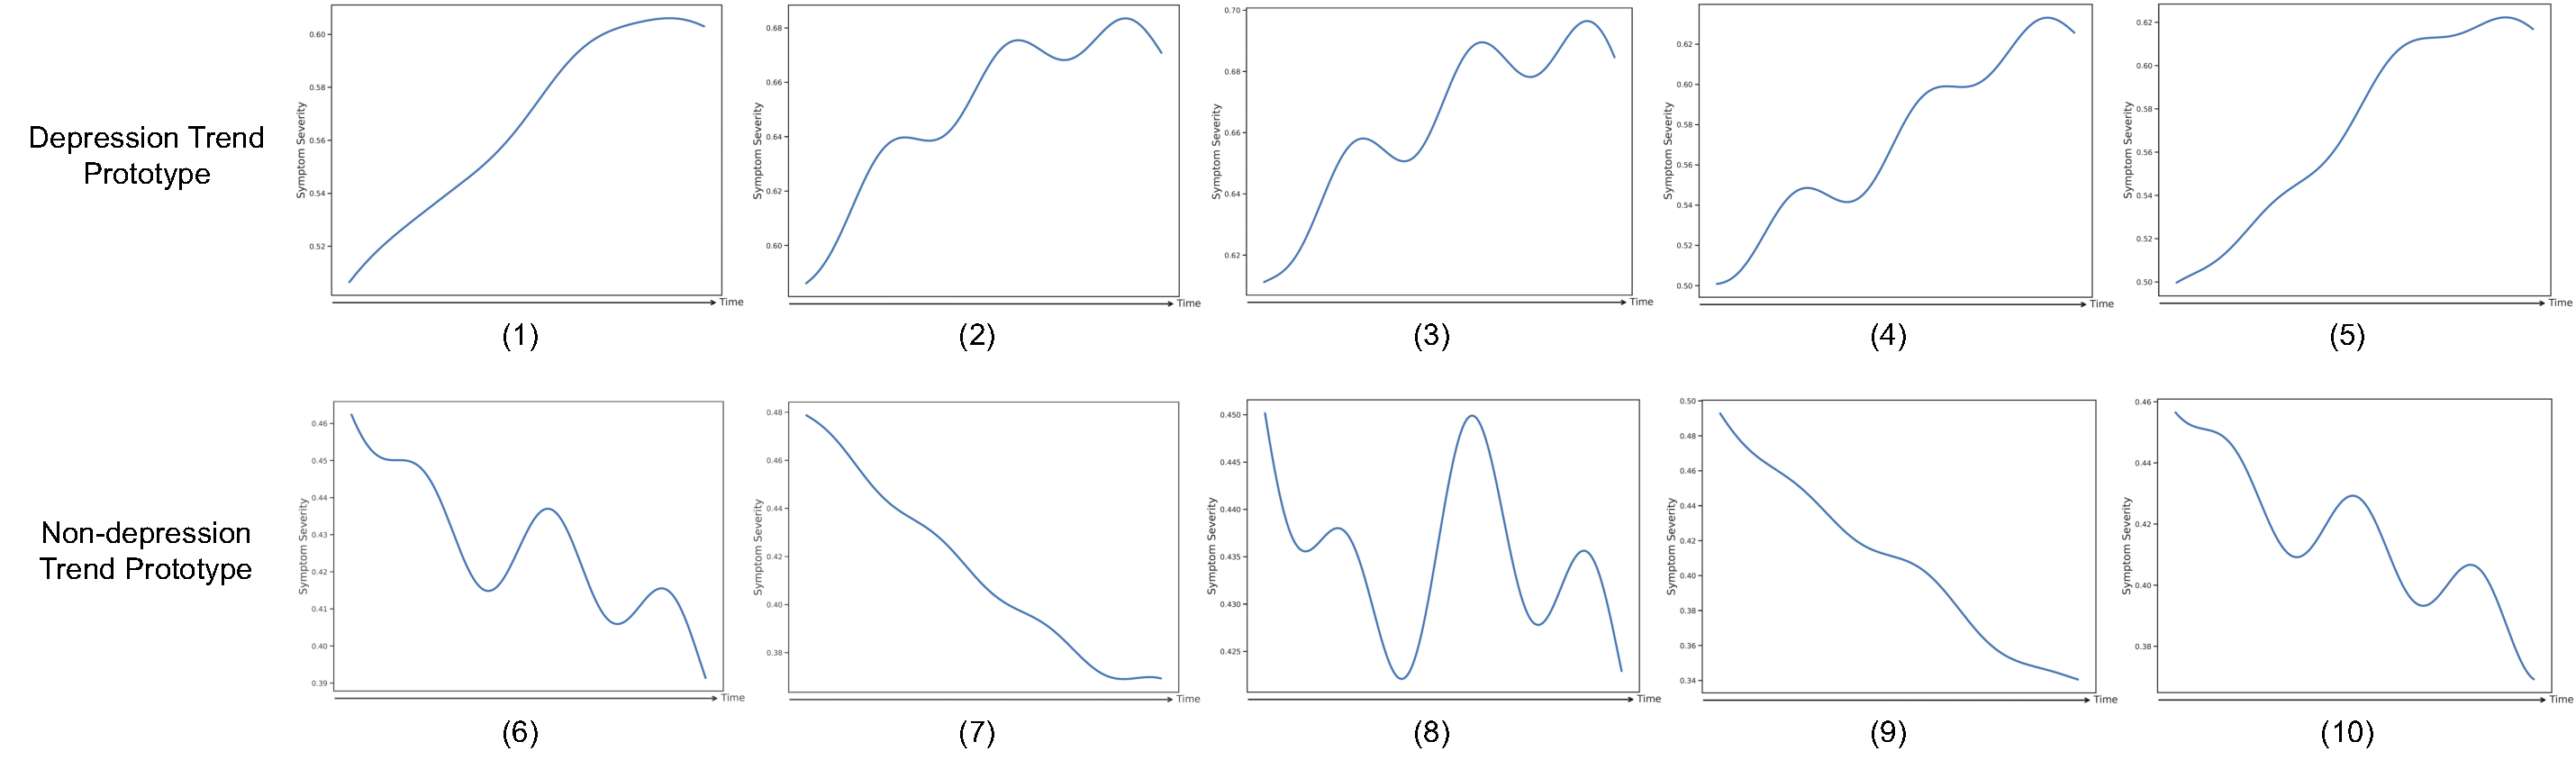
\includegraphics[width=1\textwidth]{imgs/trend-results.pdf}
    \caption{Trend Prototypes}
    \label{fig:trend-results}
\end{figure}

Trend prototypes (1)-(5) are depression trend prototypes. They represent the severities of depression symptoms trending up. Some of them have deviations from time to time in the upward trend, such as (2)-(4), representing temporary symptom relief and deterioration of depression. This conforms with the typical depression trend \citep{bockting_lifetime_2015}. Trend prototypes (6)-(10) are non-depression trend prototypes, where (6), (7), (9), and (10) represent trending down and (8) represents fluctuating with no trend. These are not typical depression trends. Each trend prototype is coupled with underlying symptoms. Figure \ref{fig:symptom-results} shows the symptom prototypes that our model learned.

\begin{figure}[h]
    \centering
    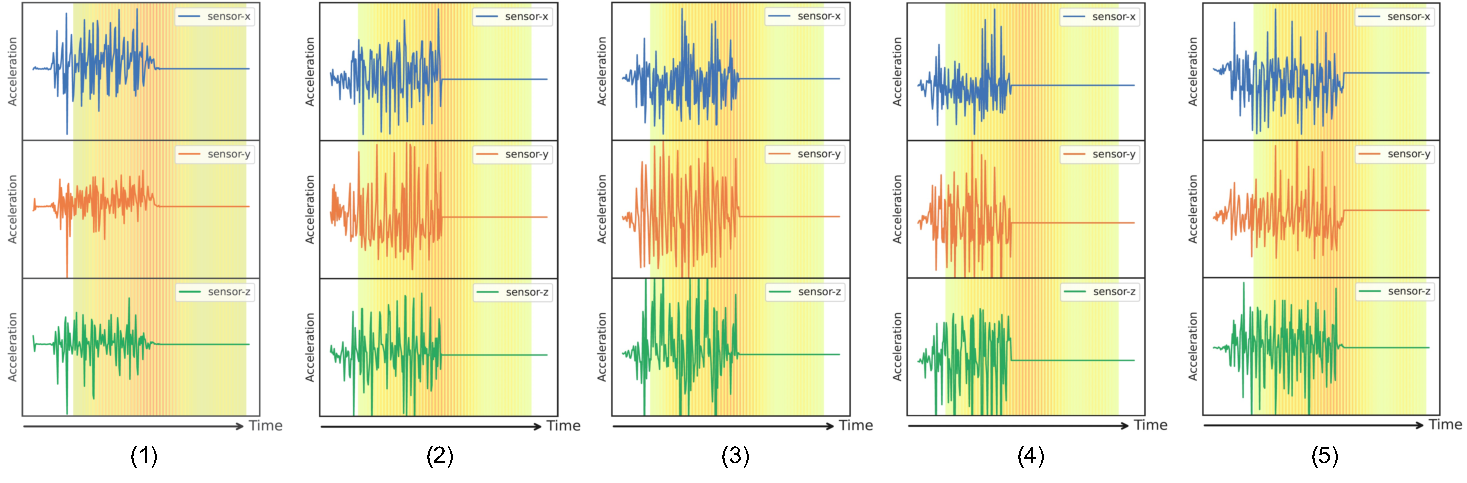
\includegraphics[width=1\textwidth]{imgs/symptom-result.pdf}
    \caption{Symptom Prototypes}
    \label{fig:symptom-results}
\end{figure}

The prototype visualization in Figure \ref{fig:symptom-results} shows the sensor signal of the symptoms. Prior literature suggests that depression walking symptoms can be reflected in gait features, such as walking speed, stride, and speed of the lifting motion of the leg \citep{sloman_gait_1982,lemke_spatiotemporal_2000,nhs_symptoms_2022}. When interpreting the prediction of a patient, these gait features can be computed for the symptom prototypes. The yellow area is the receptive field that presents the corresponding symptom. The darker the color, the stronger the symptom is present in that region.

Leveraging the above-learned trend prototypes and symptom prototypes, our model can interpret the prediction of depression for every patient. We randomly select two patients (one depressed and one non-depressed) and showcase TempPNet's interpretation for them. Figure \ref{fig:interpret-depression} shows the interpretation of the depressed patient, and Figure \ref{fig:interpret-nondepression} shows the interpretation of the non-depressed patient. For simplicity, we only show the trend prototype with the highest existing strength and the corresponding symptom prototype with the highest existing strength in these examples. For the symptom prototype, we also compute the gait features using the GaitPy package\footnote{\url{https://pypi.org/project/gaitpy/}} to explain the encoded information from the visualization.

\begin{figure}[h]
    \centering
    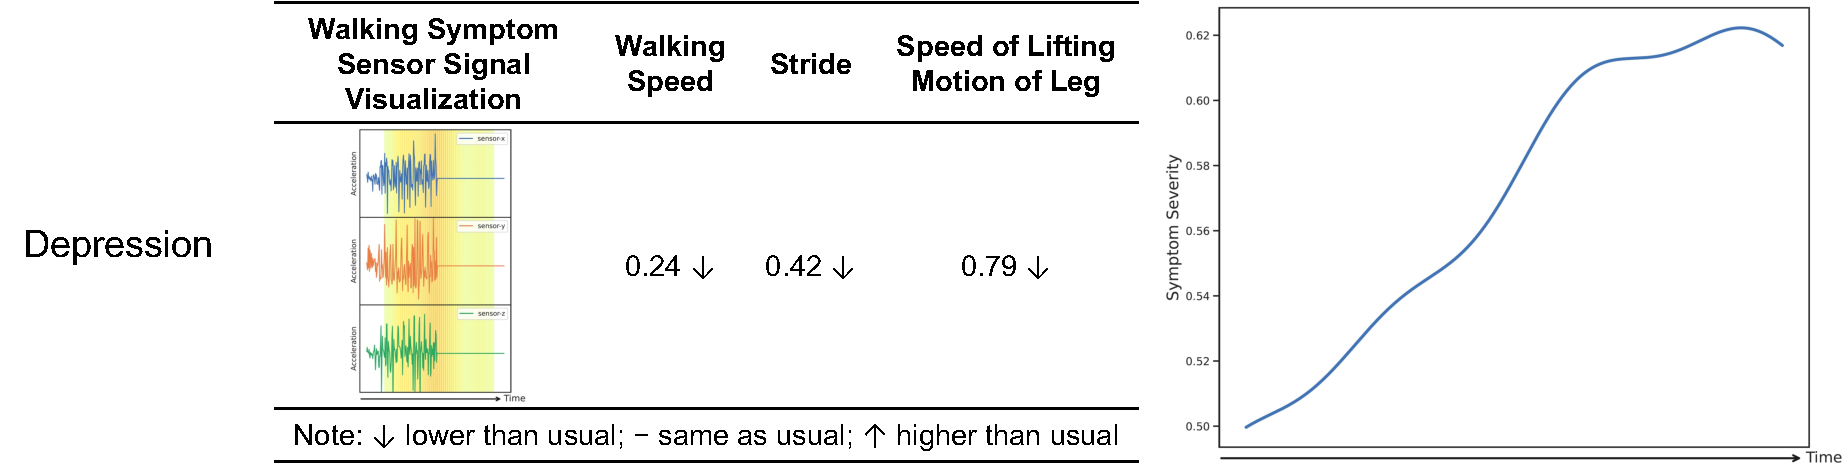
\includegraphics[width=0.8\textwidth]{imgs/interpret-depression.pdf}
    \caption{Interpretation of A Depressed Patient}
    \label{fig:interpret-depression}
\end{figure}

\begin{figure}[h]
    \centering
    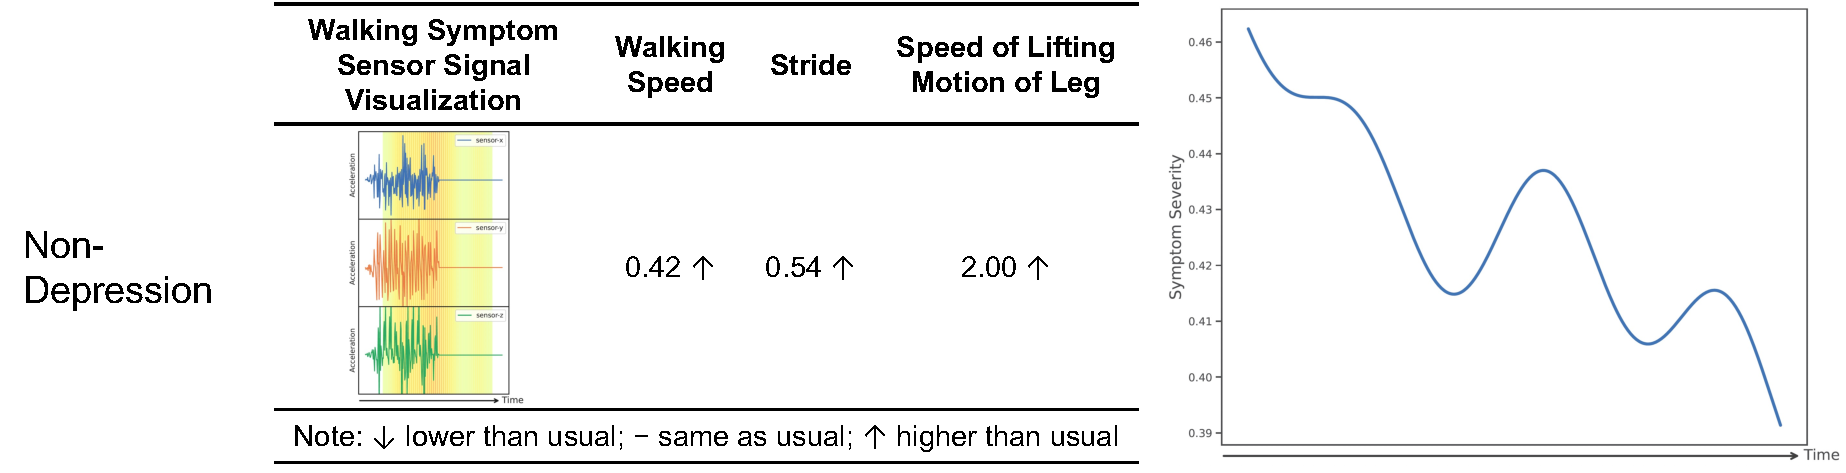
\includegraphics[width=0.8\textwidth]{imgs/interpret-nondepression.pdf}
    \caption{Interpretation of A Non-depressed Patient}
    \label{fig:interpret-nondepression}
\end{figure}

TempPNet predicts the patient in Figure \ref{fig:interpret-depression} as depressed for two reasons. First, this patient's walking patterns strongly present a walking symptom like in the left part of Figure \ref{fig:interpret-depression}. This walking symptom is manifested as slower-than-usual walking speed\footnote{The usual case is computed as the mean of each gait feature among the non-depressed participants in the dataset.}, shorter stride, and slower lifting motion of the leg. This symptom conforms with the depression physical symptoms in the literature \citep{sloman_gait_1982,lemke_spatiotemporal_2000,nhs_symptoms_2022}. Second, the severity of the previously mentioned symptom presents a temporal progression pattern like the right part of Figure \ref{fig:interpret-depression}. TempPNet believes this temporal symptom progression pattern resembles a typical depression progression pattern. According to the depression progression literature \citep{bockting_lifetime_2015,dattani_mental_2021}, this judgment makes sense — this patient's depression walking symptom first worsens rapidly and then peaks, similar to the onset and acute phases in Figure \ref{fig:depression_trend}.

TempPNet predicts the patient in Figure \ref{fig:interpret-nondepression} as non-depressed for two reasons. First, this patient's walking patterns strongly present a walking symptom like in the left part of Figure \ref{fig:interpret-nondepression}. This walking symptom is manifested as faster-than-usual walking speed, longer stride, and faster lifting motion of the leg. This symptom does not resemble the typical depression walking symptoms in the related literature \citep{sloman_gait_1982,lemke_spatiotemporal_2000,nhs_symptoms_2022}. Second, the severity of the previously mentioned symptom presents a temporal progression pattern like the right part of Figure \ref{fig:interpret-nondepression}. The symptom severity trends down and has fluctuations in the middle. This trend does not resemble a typical depression trend.

As medical experts are aware of what a typical depression walking pattern may look like (e.g., walking symptoms and temporal symptom progression), our interpretation greatly helps doctors understand why a patient is predicted as depressed. When our interpretation matches the medical understanding, as is the case in Figures \ref{fig:interpret-depression} and \ref{fig:interpret-nondepression}, doctors would trust our model’s prediction much more. Based on our interpretation, doctors can also assess what symptoms the patient presents and in what phase of the depression progression the patient is at. This interpretation information coupled with our prediction result could subsequently inform doctors to take corresponding interventions to treat depression with increased confidence and precision.

\subsection{Human Evaluation}

The major contribution of TempPNet in interpretation lies in its capability of interpreting temporal symptom progression. To validate that capturing temporal symptom progression actually improves users' trust in our model, we conduct a user study. We recruited 80 college students and informed the participants that they would be assigned an interpretable ML model to predict depression using sensor data. We randomly selected one patient sample that the model predicted as depressed and show the participants how the model interpreted this prediction. We design two randomized groups: one to present TempPNet's interpretation, and the other to present the baseline's interpretation (without temporal symptom progression, which is equivalent to ProtoPNet).

The first part of the user study collects five control variables: age, education, gender, trust in AI, and health literacy. This user study passed randomization checks. The summary statistics and randomization \textit{p}-values are reported in Tables \ref{tb:summary_stats_cat}, \ref{tb:summary_stats_con}, and \ref{tb:randomization_check}.


\begin{table}[h]
\centering
\caption{Summary Statistics (Categorical)}
\label{tb:summary_stats_cat}
\small
\begin{threeparttable}
\begin{tabular}{L{50pt}L{60pt}C{57pt}L{50pt}L{90pt}C{57pt}}
\toprule
% \midrule
 Variable & Category & Count & Variable & Category & Count \\ 
 \midrule
 Age   & 18 and lower & 1 & Education & College freshman & 1  \\
       & 18-24 & 28 &                 & College sophomore & 9 \\
       & 25-34 & 23 &                 & College junior & 3 \\
       & 35-44 & 4 &                  & College senior & 8 \\
       & 45-54 & 2 &                  & Master & 22  \\
       & 55-64  & 2 &                 & Doctorate & 17 \\
Gender & Female & 29 & & & \\
       & Male & 31 & & & \\
 \bottomrule
\end{tabular}
\end{threeparttable}
\end{table}

\begin{table}[h]
\centering
\caption{Summary Statistics (Continuous)}
\label{tb:summary_stats_con}
\small
\begin{threeparttable}
\begin{tabular}{L{70pt}C{40pt}C{40pt}C{40pt}C{40pt}C{40pt}C{40pt}}
\toprule
% \midrule
 Statistics & Min & 1st Qu. & Median & Mean & 3rd Qu. & Max \\ \midrule
 Trust in AI & 1 & 3 & 3 & 3.2 & 4 & 4  \\
 Health Literacy & 1.250 & 2.688 & 3.000 & 3.033 & 3.500 & 4.000 \\
 \bottomrule
\end{tabular}
\end{threeparttable}
\end{table}


\begin{table}[h]
\centering
\caption{Randomization Checks}
\label{tb:randomization_check}
\small
\begin{threeparttable}
\begin{tabular}{L{40pt}C{40pt}C{40pt}C{40pt}C{70pt}C{70pt}}
\toprule
% \midrule
  & Age & Education & Gender & Trust in AI & Health Literacy \\ \midrule
 P-value & 0.893 & 0.195 & 0.958 & 0.544 & 0.788 \\
 \bottomrule
\end{tabular}
\end{threeparttable}
\end{table}


Since the interpretation is based on depression walking symptoms, we designed a depression knowledge education session for all participants. We ask the participants to read the related depression knowledge depicted in Figure \ref{fig:dep_kldg_reading}. After reading such information, they are asked to answer four questions in Figure \ref{fig:kldg_test} to test their understanding. If they answer these questions incorrectly, an error message such as in the top line of Figure \ref{fig:kldg_test} will prompt and direct them to read the information and choose again. After they answer the test questions correctly, they have sufficient knowledge to understand the model interpretations.

\begin{figure}[h]
\centering
\begin{subfigure}{0.51\textwidth}
    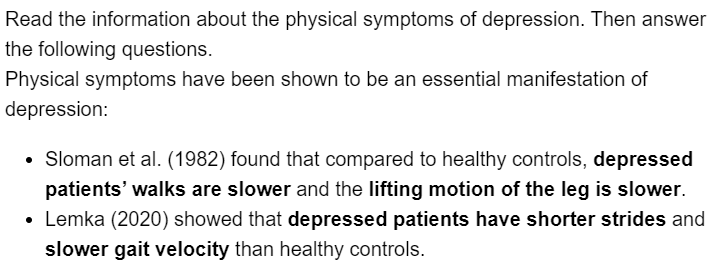
\includegraphics[width=\textwidth]{imgs/user-study-training.PNG}
    \caption{Knowledge Training Reading}
    \label{fig:dep_kldg_reading}
\end{subfigure}
\hfill
\begin{subfigure}{0.37\textwidth}
    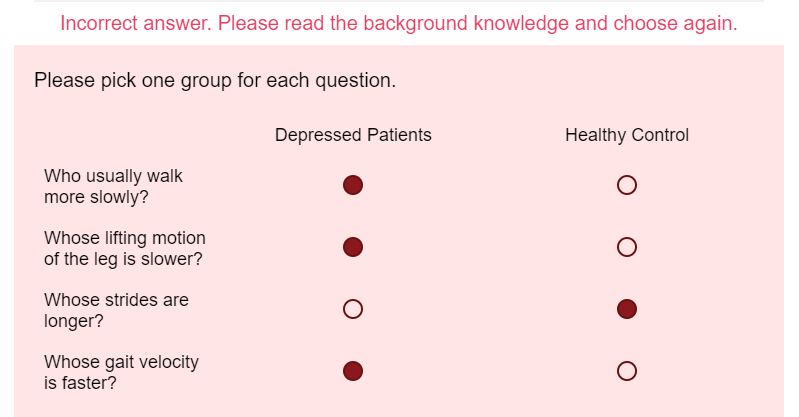
\includegraphics[width=\textwidth]{imgs/training-question.PNG}
    \caption{Knowledge Training Test}
    \label{fig:kldg_test}
\end{subfigure}
\caption{Depression Knowledge Training}
\label{fig:dep_kldg_training}
\end{figure}

In the next part of the user study, we inform the participants the prediction context, input, and output. Then, we show the model interpretation to each group respectively, as shown in Figure \ref{fig:user-study-groups}. The size of the pictures is the same for both groups in the survey. A manipulation check question is asked to verify whether the participants read the interpretation carefully (``How does the walking speed of the above walking symptom compare to the usual case?''), whose answer can be understood from the arrow sign after the value of the walking speed in the interpretation figure. Subsequently, we ask the participants to rate their trust in the given model. The measurement scale is adopted from \cite{chai_factors_2011}. The Chronbach's Alpha is 0.901 for this scale, suggesting excellent reliability. The factor loadings of the scale are reported in Appendix \ref{apd:trust_factor_loading}, suggesting good validity. In this scale, an attention check question is added (``Please just select neither agree nor disagree.''). After removing the participants who failed the attention check or the manipulation check, 60 participants remain in the final analyses. Figure \ref{fig:user-study-trust} shows the mean of trust for each of the two groups. The participants' trust in our model (mean = 2.31) is significantly higher than the baseline model (mean = 1.65, \textit{p} < 0.001). This result indicates that interpreting the temporal symptom progression is a critical booster for users' trust in depression prediction models, endorsing our model design.
 
\begin{figure}[H]
\centering
\begin{subfigure}{0.59\textwidth}
    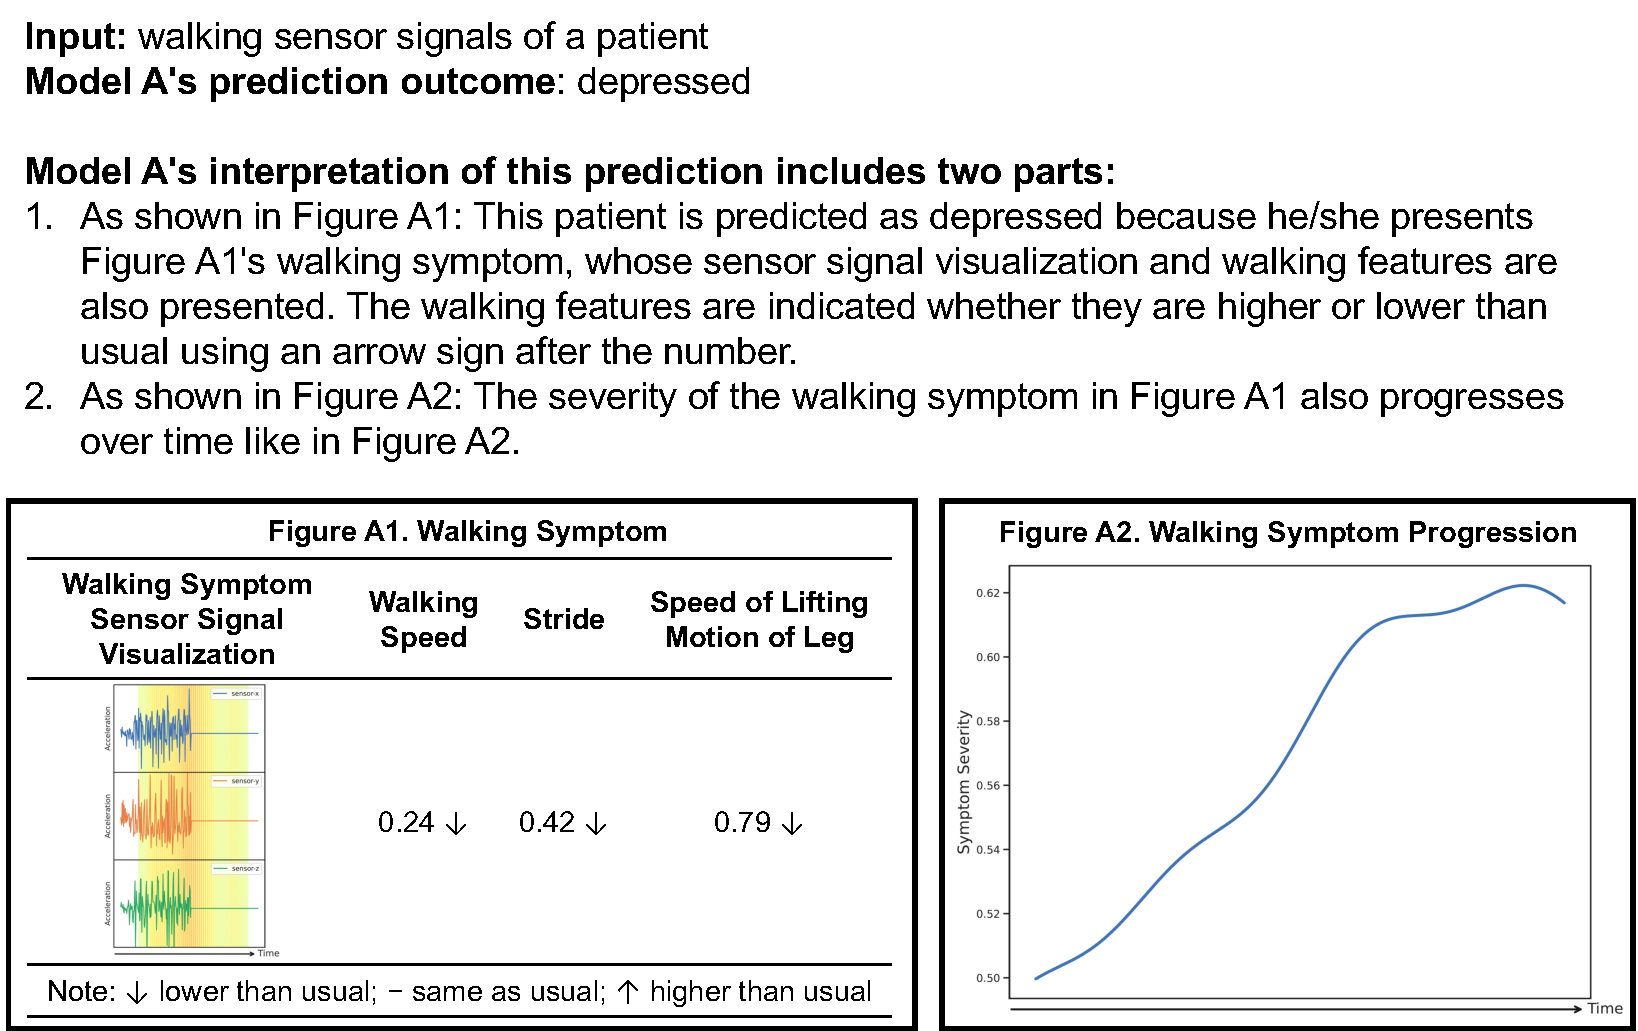
\includegraphics[width=\textwidth]{imgs/user-study-temppnet.pdf}
    \caption{Group TempPNet}
    \label{fig:user-study-temppnet}
\end{subfigure}
% \hfill
\begin{subfigure}{0.4\textwidth}
    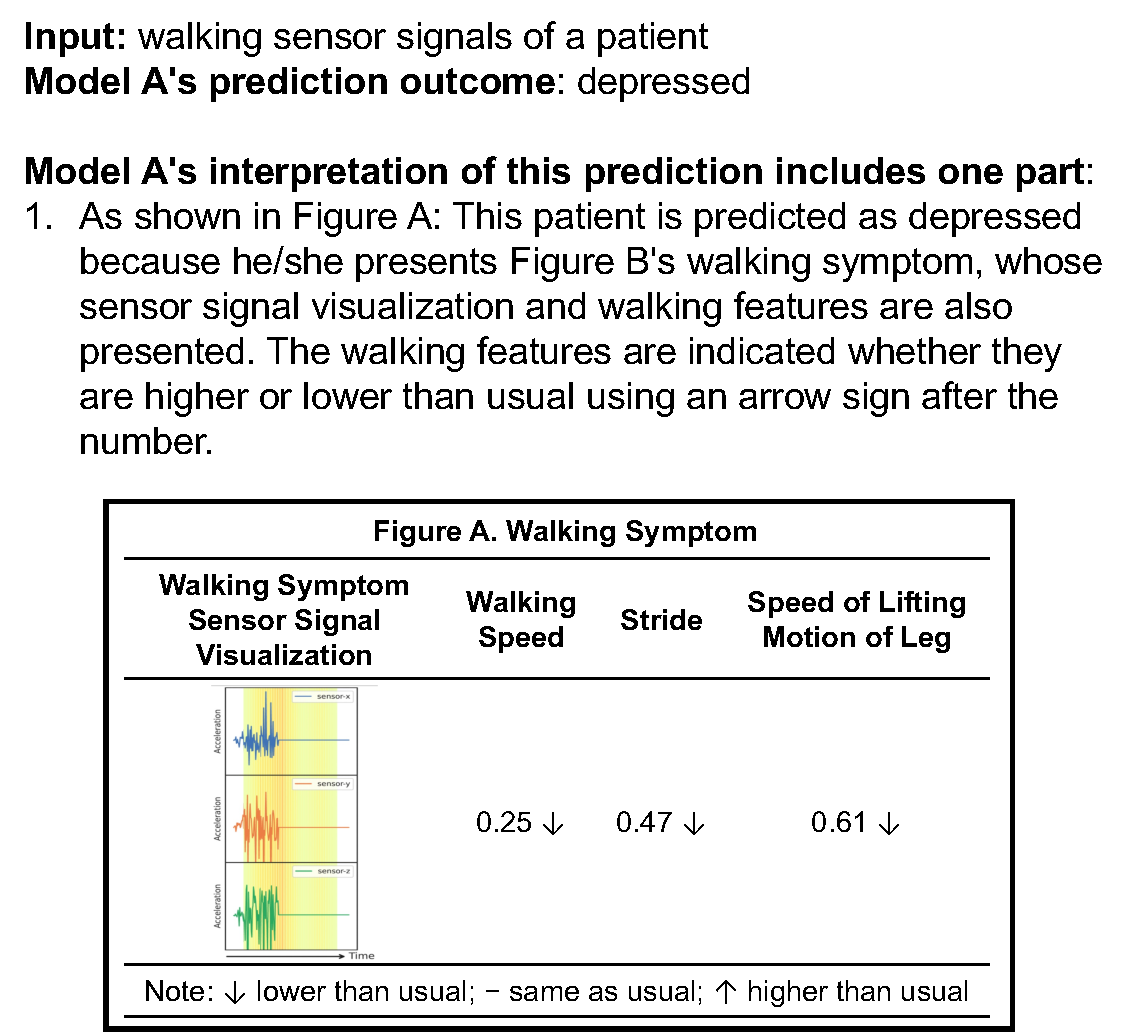
\includegraphics[width=\textwidth]{imgs/user-study-protopnet.pdf}
    \caption{Group Baseline}
    \label{fig:user-study-protopnet}
\end{subfigure}
\caption{User Study Groups}
\label{fig:user-study-groups}
\end{figure}

\begin{figure}[h]
    \centering
    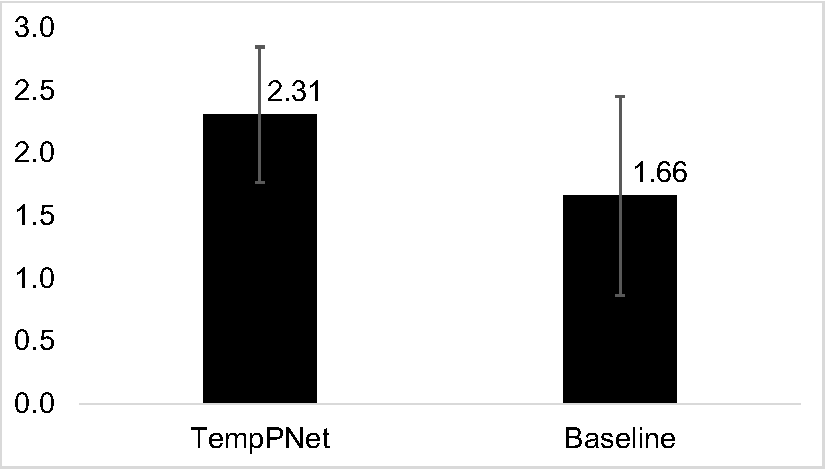
\includegraphics[width=0.4\textwidth]{imgs/user-study-trust.pdf}
    \caption{Trust Comparison Between TempPNet and Baseline}
    \label{fig:user-study-trust}
\end{figure}

After the participants rate the trust for the given model, we then show them the interpretation of the other model as a comparison. We ask them to choose a model interpretation that they trust more. 50 participants (83.3\%) chose TempPNet over the baseline. When asked why they trust TempPNet more than the baseline, 31 participants mentioned, in similar wording, that ``because this model visualized the walking symptom progression.'' The above user study results prove that by interpreting the temporal symptom progression, TempPNet improves users' trust in our model, which offers empirical evidence for the contribution of our model innovation.

\section{Discussion and Conclusions} \label{sec:discuss}

Depression prediction is fundamental to comprehensive chronic care in the health sensing area. Although a few studies tapped this domain, they do not offer a meaningful interpretation of their predictions. Prototype learning methods, a class of state-of-the-art interpretable methods, fall short in modeling the temporal progression of depression. To address these limitations, we propose a novel interpretable deep learning method to predict depression using sensor data while interpreting its predictions based on the temporal progression of depression. We conduct extensive evaluations to demonstrate superior predictive power of our method over state-of-the-art benchmarks and showcase its interpretation of predictions. Furthermore, through a user study, we show that our method outperforms these benchmarks in terms of interpretability. 

Our study contributes to the extant literature in two aspects. First, our work belongs to the computational genre of design science research, which develops computational methods to solve business and societal problems and aims to make methodological contributions \citep{rai_editors_2017,Simchi-Levi_2020,padmanabhan_machine_2022}. In this regard, our proposed TempPNet is a novel prototype learning method that processes a sequence of inputs and interprets predictions based on prototypes of temporal symptom progression. To design TempPNet, we innovatively overcome three methodological challenges: learning prototypes of depression symptoms, learning prototypes of  temporal symptom progression from walking tests performed at irregular time intervals, and modeling walking tests of varying lengths. Second, our study contributes to healthcare IS research with a novel interpretable deep learning method that predicts depression associated with chronic diseases using motion sensor data and interprets its predictions.


\subsection{Research and Practical Implications}


This study has implications for predictive and prescriptive analytics research. Over the years, methods that predict future actions (i.e., predictive analytics) or specify optimal decisions (i.e., prescriptive analytics) have been developed to solve problems in a diverse set of domains such as health analytics, video analytics, and social media analytics \citep{xie_unbox_2020,yu_wearable_2022}.
Our proposed method is particularly useful for those models that rely on snapshot information to make a prediction but neglect the temporal changes of such information. For example, one closely related area that TempPNet can be generalized to is Parkinson's disease (PD) progression prediction and interpretation. Similar to our study, motion sensor data can be collected to reflect the motion symptoms of PD. The symptom prototype of our method can detect typical PD walking symptoms, such as smaller steps, slower speed, less trunk movement, and a narrow base of support.\footnote{\url{https://www.parkinson.org/understanding-parkinsons/symptoms/movement-symptoms/trouble-moving}} PD patients' symptoms may also form a trend. The trend prototype of our method is able to detect such a trend, predict PD severity, and interpret such a prediction.

Consider another application area, as sensor data naturally resemble image data, TempPNet can be used to process time-series images, or videos. The applicable tasks include object detection, video classification, among others. The symptom prototype in our method can be adapted to recognize typical objects in each video frame, and the trend prototype can be used to capture the temporal changes of these objects, such as shape and angle changes, location moves, and context shifts. Beyond the above-mentioned applications, TempPNet can be generalized to interpretable prediction problems where the temporal progression of information is essential.


Our proposed method holds significant practical implications. For doctors, our method can be deployed in mobile applications. Doctors can encourage their chronic disease patients to install these applications to actively monitor patients' walking data. Our method is able to predict the depression risk on a daily basis. When our method signals a high depression risk, the doctors could review the interpretation given by our model and understand what depression walking symptoms the patient presents and how the patient's depression severity has progressed over time. Timely and personalized interventions can be taken to prevent the deterioration of depression and the negative spill-over effects for physical chronic symptom treatments. For caregivers, our method offers an opportunity to keep track of the daily mental health updates of their loved ones. When the mental health deteriorates, the caregivers can actively seek medical help, provide emotional support, and look for social support groups for the patients. For patients, our method can provide a daily health check dashboard, so that they are aware of their mental health status. For the healthcare system, since depression poses a significant economic burden, our method enables active monitoring of depression and timely intervention, thus greatly reducing the preventable mental illness costs and related complications for the linked main chronic disease treatment.

\subsection{Limitations and Future Research}

Our study has a few limitations and can be extended in multiple directions. First, our walking signals are collected via walking tests from the mPower study \citep{bot_mpower_2016}. Although clinical studies have proven that walking tests are a reliable test for assessing functional symptoms of depressed patients \citep{vancampfort_testretest_2020}, continuous collection of sensor signals could provide a richer reflection of depression symptoms. Nevertheless, continuous sensor data collection while matching the scale of the mPower study necessitates significant costs, including mobile application development, recruiting and obtaining consent from participants, and data storage, among others. If budgets permit, future studies can conduct natural experiments to collect continuous sensor data for chronic disease patients and improve the training data of our model. Second, similar to any experimental studies, it is likely that participants may attempt to perform a desired behavior in the walking test that they would not normally do in real life. This issue is mitigated in this study. The mPower study is a longitudinal study with a general purpose of health management for chronic disease patients. Patients are not anchored to change any behavior related to depression. Besides, this study focuses on major depressive disorder which is persistent and has significant impairment \citep{mayo_clinic_depression_2022}, instead of temporary mood swings. Such persistent symptoms are difficult to self-control. Because of that, \cite{vancampfort_testretest_2020} have proved that self-conducted walking tests can reliably reveal the physical symptoms of depression. Even in professional clinical settings, many disorders involving movement impairment, such as Parkinson's disease, are also diagnosed via walking tests in the doctor's office \citep{yu_wearable_2022}. If research budgets are available, future studies could collect the sensor data continuously without having to initiate the test setting.

% ---------------- main paper bib ------------------------

\bibliographystyle{informs2014} % outcomment this and next line in Case 1
\bibliography{Project-IDDvSD} % if more than one, comma separated
\clearpage

\renewcommand{\theequation}{\arabic{equation}} 
\renewcommand{\thetable}{\arabic{table}}

\ECSwitch

\ECHead{Supplementary Materials}

\begin{appendices}

% \setcounter{algorithm}{0}
% \renewcommand\thealgorithm{A.\arabic{algorithm}}


\section{The Definition of Sensor Features}\label{apd:sen_features}

We explain the content of a sensor feature as mentioned in Section \ref{sec:problem_formulation}.
At each timepoint $l$, the mobile sensor collects accelerometer readings $[x_l^{\mathfrak{L}},y_l^{\mathfrak{L}},z_l^{\mathfrak{L}}]$ and orientation readings $[x_l^{o},y_l^{o},z_l^{o},w_l^{o}]$. A graphic illustration of these sensor readings is shown in Figure \ref{fig:frame_change}.
\begin{figure}[h]
    \centering
    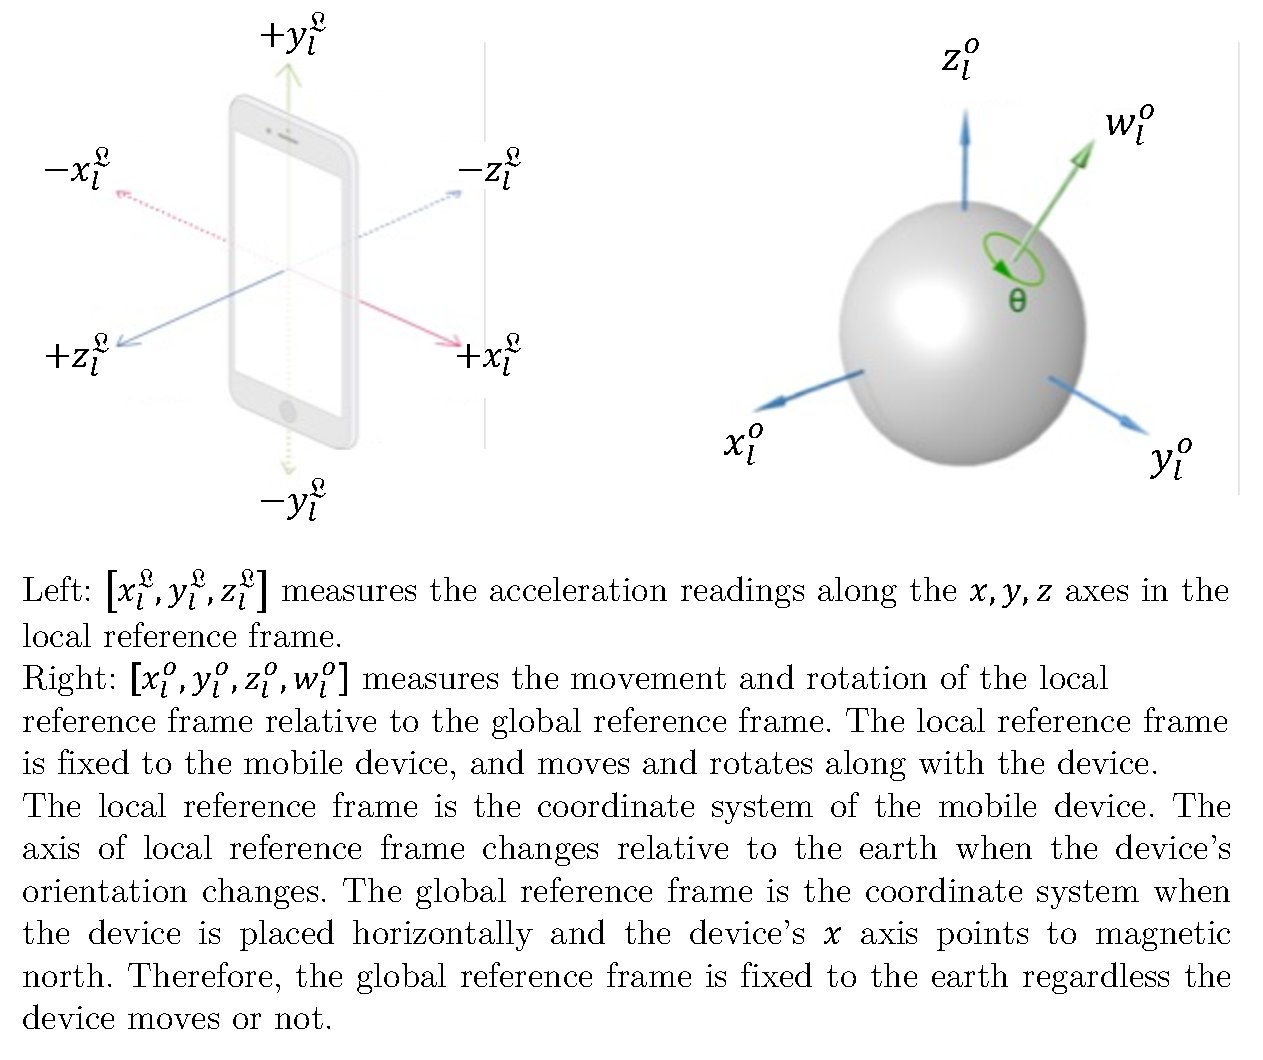
\includegraphics[width=0.7\textwidth]{imgs/frame_change.pdf}
    \caption{Sensor Readings \citepsec{apple_inc_understanding_2022_a} }
    \label{fig:frame_change}
\end{figure}

The accelerometer readings are in the local reference frame, which most existing studies rely on \citepsec{piau_when_2020_a,yu_wearable_2022_a,zhu_deep_2021_a}. However, these local reference readings do not reflect the precise walking pattern in the geographic coordinate system, because it moves and rotates along with the mobile device. To address this issue and make the interpretation more meaningful in the geographic sense, we decide to work with the readings in the global reference frame. We transform the local reference frame accelerometer vector $v_l^{\mathfrak{L}} =[x_l^{\mathfrak{L}},y_l^{\mathfrak{L}},z_l^{\mathfrak{L}}]^T$ to the global reference frame as $v_l^\mathfrak{G} =[x_l^{\mathfrak{G}},y_l^{\mathfrak{G}},z_l^{\mathfrak{G}}]^T$ via the quaternion rotation 
$$v_l^{\mathfrak{G}} = \mathcal{R}_l v_l^{\mathfrak{L}}$$ 
where $\mathcal{R}_l$ is the rotation matrix derived from quaternion $[x_l^{o},y_l^{o},z_l^{o},w_l^{o}]$ as follows. In general, given a quaternion $[x,y,z,w]$, the corresponding rotation matrix $\mathcal{R}$ is defined as\footnote{\url{https://en.wikipedia.org/wiki/Quaternions_and_spatial_rotation}}
\begin{equation}
\label{eq:rotation_matrix}
   \mathcal{R} = \begin{bmatrix}
       w^2+x^2-y^2-z^2 & 2 x y-2w z & 2 x z+2 w y \\  
        2 x y+2 w z & w^2-x^2+y^2-z^2 & 2 y z-2w x \\
       2 x z-2w y & 2 y z + 2 w x & w^2 - x^2- y^2 + z^2
   \end{bmatrix}.
\end{equation}
Then, we define the sensor feature $a_l$ as
\begin{equation}
a_{l}=[x_l^{\mathfrak{G}},y_l^{\mathfrak{G}},z_l^{\mathfrak{G}} ]^T.
\end{equation}

Following the best practice of data augmentation for mobile sensor data \citepsec{um_data_2017_a,zhang_deep_2020_a}, during the training stage, we further transform the input sensor features with random rotations to improve the generalization ability of our model. To do this, we first sample a quaternion using Algorithm \ref{alg:sample_quaternion} where $\text{Uniform}(b_1,b_2)$ means the uniform distribution on the interval $[b_1,b_2]$, and then plug the obtained quaternion into Equation \ref{eq:rotation_matrix} to construct a random rotation matrix. Within each training epoch and for each walking test, we construct a random rotation matrix $\tilde{\mathcal{R}}$ as described, and then use it to transform all sensor features of the walking test as $\langle \tilde{\mathcal{R}} a_1, \tilde{\mathcal{R}} a_2, \dots, \tilde{\mathcal{R}} a_L \rangle$. Once the training stage is finished, we use the original sensor features $\langle a_1, a_2, \dots, a_L \rangle$ to do inference.

\begin{algorithm}[h]
% \small
\caption{Sample a Quaternion}\label{alg:sample_quaternion}
\begin{algorithmic}[1]
\State Draw $x \sim \text{Uniform}(0,1)$, $y \sim \text{Uniform}(0,1)$, $z \sim \text{Uniform}(0,1)$.
\State Let $\text{norm}=\sqrt{x^2+y^2+z^2}$, and set $x=x/\text{norm}$, $y=y/\text{norm}$, $z=z/\text{norm}$.
\State Draw $\theta \sim \text{Uniform}(0,2\pi)$.
\State Set $w=\cos(\theta/2)$, $x=x \sin(\theta/2)$, $y=y \sin(\theta/2)$, $z=z \sin(\theta/2)$
\State Return $[x,y,z,w]$
\end{algorithmic}
\end{algorithm}

\clearpage

\section{The Specification of the Feature Extraction Layer}\label{apd:cnn}

Recall that $X_i$ denotes the sequence of sensor features of the $i$th walking test performed by a focal patient. In this section, we focus on extracting the feature matrix $H_i^\mathbb{S}$ from a single waling test, and therefore drop the subscript $i$ to simplify the notation. 
We partition $X$ into three segments according to in which task the sensor signals are recorded. Namely, $X=[X_{1}, X_{2}, X_{3}]$, which respectively denote the segment for the outbound, return, and rest (standing still) tasks. According to the definition of sensor features given in Appendix \ref{apd:sen_features}, each segment $X_j$ is in fact a matrix of size $3 \times L_j$ for $j=1,2,3$, where $L_j$ is the length of segment $j$. In general, different segments have different lengths in different walking tests. In what follows, we assume that $X$ has been downsampled with the frequency of 10 Hz, while the treatment of other sampling frequencies should be adjusted proportionally.

Under the sampling frequency of 10 Hz, we observe that the rest segment on average has the longest sequence, with $L_3=296$ by averaging over all walking tests. To facilitate batch training, we reshape each segment into a matrix of size $3 \times 300$, by either padding it with zero columns if its length is smaller than $300$, or discarding the extra columns if its length is larger than $300$.
After the reshaping step, we treat each segment $X_j$ as an input of $3$ channels and length $300$, and then use the same CNN layer to extract a feature matrix of size $128 \times 5$ from $X_j$. The CNN layer is composed by a sequence of one-dimensional convolution (Conv1d) layers, each followed in order by a one-dimensional batch normalization layer (BatchNorm1d), a max pooling layer (MaxPool1d), and lastly a leaky ReLU layer (LeakyReLU) with slope $0.01$ for non-linear activation \citepsec{goodfellow_deep_2016_a}. Following the style of \citesec{zhu_deep_2021_a}, we report the detailed architecture of the CNN layer in Table \ref{tb:cnn_layer}. Since the BatchNorm1d layer and the LeakyReLU layer do not change the input shape, we do not list them in Table \ref{tb:cnn_layer}. After the last Conv1d layer in Table \ref{tb:cnn_layer}, we do not add the MaxPool1d layer nor the LeakyReLU layer.

\begin{table}[h]
\centering
\caption{The Specification of the CNN Layer}
\label{tb:cnn_layer}
\small
\begin{threeparttable}
\begin{tabular}{L{50pt}C{40pt}C{30pt}C{40pt}C{60pt}}
\toprule
% \midrule
 & Kernel Size & Stride & Output Channel & Output Shape \\ \midrule
 % Input & & & 3 & (3, 300) \\
 Conv1d & 8 & 1 & 256 & (256, 293) \\
 MaxPool1d & 2 & 2 & & (256, 146) \\
 
 Conv1d & 8 & 1 & 512 & (512, 139) \\
 MaxPool1d & 2 & 2 & & (512, 69) \\
 
 Conv1d & 8 & 1 & 256 & (256, 62) \\
 MaxPool1d & 2 & 2 & & (256, 31) \\
 
 Conv1d & 8 & 1 & 128 & (128, 24) \\
 MaxPool1d & 2 & 2 & & (128, 12) \\
 
 Conv1d & 8 & 1 & 128 & (128, 5) \\
 \bottomrule
\end{tabular}
\end{threeparttable}
\end{table}

Given the input $X=[X_1,X_2,X_3]$, we feed each segment $X_j$ into the same CNN layer specified above, and obtain a feature matrix $H_j^\mathbb{S}$ of size $128 \times 5$ for $j=1,2,3$. We then horizontally concatenate these feature matrices to obtain the final feature matrix as $H^\mathbb{S}=[H_1^\mathbb{S}, H_2^\mathbb{S}, H_3^\mathbb{S}]$ of size $n_e \times n_o$, where $n_e=128$ and $n_o=15$.

\clearpage

\section{The Density Function of the Logistic-Normal Distribution}\label{apd:der_logistic_normal}

We employ the change of variables formula \citepsec{murphy_probabilistic_2022_a} to derive Equation \ref{eq:sigmoid_gauss_density}, which in general states that if a random vector $x \in R^{M}$ is mapped to another random vector $z \in R^{M}$ by an invertible
function $f$, i.e., $z=f(x)$, then the density function of $z$, denoted by $p_z(z)$, is related to the density function of $x$, denoted by $p_x(x)$, by the following relationship:
\begin{equation}
\label{eq:change_of_var}
p_z(z) = p_x\big( g(z) \big) \big| \det[J_g(z)] \big|
\end{equation}
where $g$ is the inverse function of $f$, $J_{g}(z) \in R^{M \times M}$ is the Jacobian matrix of $g$ evaluated at $z$, $\det [.]$ is the matrix determinant operator, and $|.|$ is the absolute value operator. 

In our case, $z=\sigma(x)$, which means that $f=\sigma$ and $g=\sigma^{-1}$. Using the fact that $\partial x_m/\partial z_m = 1 / (z_m(1-z_m))$, the corresponding Jacobian matrix can be computed as
\begin{equation}
% \label{eq:jacobian}
J_{g}(z) =  \begin{pmatrix}
    \frac{1}{z_1 (1-z_1)} & 0 & \dots & 0 \\
    0 & \frac{1}{z_2 (1-z_2)} & \dots & 0 \\
    \vdots & \vdots & \ddots & \vdots \\
    0 & 0 & \dots & \frac{1}{z_M (1-z_M)}
  \end{pmatrix},
\end{equation}
which is a diagonal matrix because $\sigma^{-1}$ has been element-wisely applied on $z$. Given that $0< z_m < 1$ for $m=1,2,\dots,M$, all the diagonal elements are positive, and thus we have 
\begin{equation}
\label{eq:jacobain_det}
   \big| \det[J_g(z)] \big|  = \frac{1}{\prod_{m=1}^{M} z_{m}(1-z_{m})}.
\end{equation}
Recall that $x \sim \mathcal{N}(\mu, \Sigma)$, then the corresponding density function is given by 
\begin{equation}
\label{eq:gauss_density}
p_x(x) = \frac {\exp \big(-\frac{1}{2}(x-\mu)^{T}{\Sigma}^{-1}(x-\mu) \big)}{ \sqrt{(2 \pi)^{M} \det[\Sigma] }}.
\end{equation}
Plugging Equation \ref{eq:jacobain_det} and \ref{eq:gauss_density} into Equation \ref{eq:change_of_var}, and setting $x=\sigma^{-1}(z)$, we obtain Equation \ref{eq:sigmoid_gauss_density}.

\clearpage

\section{Manually Crafted Features for Benchmarks}\label{apd:mannual_features}

Recall that given a walking test, we observe a sequence of sensor signals $\langle v_1^{\mathfrak{L}}, v_2^{\mathfrak{L}}, \dots, v_L^{\mathfrak{L}} \rangle$, where $v_l^{\mathfrak{L}}$ is the accelerometer readings recorded in the local reference frame at timepoint $l$, as explained in Appendix \ref{apd:sen_features}. To simplify notation, we drop the superscript $\mathfrak{L}$, and write $v_l=[v_{x,l},v_{y,l},v_{z,l}]^T$.
Following \citesec{yu_wearable_2022_a}, we define the following features for each given walking test. 

\begin{table}[h]
\centering
\caption{Features for Conventional Machine Learning Models}
\label{tb:baseline_features}
\small
\begin{threeparttable}
\begin{tabular}{L{160pt}L{290pt}}
\toprule
% \midrule
 Feature Name & Formula \\ \midrule
 Mean x-axis values &  $u_{x} = \frac{1}{L} \sum_{l=1}^{L} v_{x,l}$ \\
 Mean y-axis values &  $u_{y} = \frac{1}{L} \sum_{l=1}^{L} v_{y,l}$ \\
 Mean z-axis values &  $u_{z} = \frac{1}{L} \sum_{l=1}^{L} v_{z,l}$ \\
 St. D. of x-axis values &  $\sigma_{x} = \sqrt{\frac{1}{L-1} \sum_{l=1}^{L} (v_{x,l} - u_{x} )^2 } $ \\
 St. D. of y-axis values &  $\sigma_{y} = \sqrt{\frac{1}{L-1} \sum_{l=1}^{L} (v_{y,l} - u_{y} )^2 } $ \\
 St. D. of z-axis values &  $\sigma_{z} = \sqrt{\frac{1}{L-1} \sum_{l=1}^{L} (v_{z,l} - u_{z} )^2 } $ \\
 Mean magnitude &  $u_{v} = \frac{1}{L} \sum_{l=1}^{L} ||v_l||$, $||v_l||=\sqrt{v_{x,l}^2+v_{y,l}^2+v_{z,l}^2} $ \\
 St. D. of magnitude &  $\sigma_{v} = \sqrt{\frac{1}{L-1} \sum_{l=1}^{L} (||v_l|| - u_v)^2 } $ \\
 Mean x-axis jerk & $\alpha_{x} = \frac{1}{L-1} \sum_{l=1}^{L-1} d_{x,l}$, where $d_{x,l}=v_{x,l+1}-v_{x,l}$ \\
 Mean y-axis jerk & $\alpha_{y} = \frac{1}{L-1} \sum_{l=1}^{L-1} d_{y,l}$, where $d_{y,l}=v_{y,l+1}-v_{y,l}$  \\
 Mean z-axis jerk & $\alpha_{z} = \frac{1}{L-1} \sum_{l=1}^{L-1} d_{z,l}$, where $d_{z,l}=v_{z,l+1}-v_{z,l}$  \\
 St. D. of x-axis jerk &  $\beta_{x} = \sqrt{\frac{1}{L-2} \sum_{l=1}^{L-1} (d_{x,l} - \alpha_{x} )^2 } $ \\
 St. D. of y-axis jerk &  $\beta_{y} = \sqrt{\frac{1}{L-2} \sum_{l=1}^{L-1} (d_{y,l} - \alpha_{y} )^2 } $ \\
 St. D. of z-axis jerk &  $\beta_{z} = \sqrt{\frac{1}{L-2} \sum_{l=1}^{L-1} (d_{z,l} - \alpha_{z} )^2 } $ \\
 Mean jerk magnitude &  $\alpha_{d} = \frac{1}{L-1} \sum_{l=1}^{L-1} ||d_l|| $, where $||d_l||=\sqrt{d_{x,l}^2+d_{y,l}^2+d_{z,l}^2}$ \\
 St. D. of jerk magnitude & $\beta_{d} = \sqrt{\frac{1}{L-2} \sum_{l=1}^{L-1} (||d_l|| - \alpha_{d})^2 } $  \\
 Stride time variability on x-axis & \multicolumn{1}{p{290pt}}{
 (1) Identify signal peaks in x-axis, $[t_1,t_2,\dots,t_Q]$;\newline 
 (2) Identify stride times $[d t_1,d t_2,\dots,d t_{Q-1}]$, where $d t_i=t_{i+1}-t_i$; \newline 
 (3) Compute stride time variability $V_{x}=\sqrt{\frac{1}{Q-2} \sum_{i=1}^{Q-1} (d t_i - \overline{d t} )^2 }$ }  \\
 Stride time variability on y-axis & \multicolumn{1}{p{290pt}}{
 (1) Identify signal peaks in y-axis, $[t_1,t_2,\dots,t_Q]$;\newline 
 (2) Identify stride times $[d t_1,d t_2,\dots,d t_{Q-1}]$, where $d t_i=t_{i+1}-t_i$; \newline 
 (3) Compute stride time variability $V_{y}=\sqrt{\frac{1}{Q-2} \sum_{i=1}^{Q-1} (d t_i - \overline{d t} )^2 }$ }  \\
 Stride time variability on z-axis & \multicolumn{1}{p{290pt}}{
 (1) Identify signal peaks in z-axis, $[t_1,t_2,\dots,t_Q]$;\newline 
 (2) Identify stride times $[d t_1,d t_2,\dots,d t_{Q-1}]$, where $d t_i=t_{i+1}-t_i$; \newline 
 (3) Compute stride time variability $V_{z}=\sqrt{\frac{1}{Q-2} \sum_{i=1}^{Q-1} (d t_i - \overline{d t} )^2 }$ }  \\
 Stride time vairability on magnitude & \multicolumn{1}{p{290pt}}{
 (1) Identify signal peaks in magnitude, $[t_1,t_2,\dots,t_Q]$;\newline 
 (2) Identify stride times $[d t_1,d t_2,\dots,d t_{Q-1}]$, where $d t_i=t_{i+1}-t_i$; \newline 
 (3) Compute stride time variability $V_{v}=\sqrt{\frac{1}{Q-2} \sum_{i=1}^{Q-1} (d t_i - \overline{d t} )^2 }$ }  \\
 \bottomrule
\end{tabular}
\end{threeparttable}
\end{table}

\clearpage

\section{Factor Loadings of the Trust Scale}\label{apd:trust_factor_loading}

\begin{table}[h]
\centering
\caption{Factor Loadings of the Trust Scale}
\label{tb:factor_loading}
\small
\begin{threeparttable}
\begin{tabular}{L{60pt}C{60pt}}
\toprule
% \midrule
 Factor & Loading \\ \midrule
 Trust 1 & 0.533  \\
 Trust 2 & 0.993  \\
 Trust 3 & 0.759  \\
 Trust 4 &  0.620 \\
 Trust 5 &  0.805 \\
 Trust 6 & 0.798  \\
 Trust 7 &  0.946 \\
 Trust 8 &  0.933 \\
 Trust 9 &  0.932 \\
 \bottomrule
\end{tabular}
\end{threeparttable}
\end{table}

\clearpage


\bibliographystylesec{informs2014}
\bibliographysec{Project-IDDvSD-ap.bib} 


\end{appendices}

\end{document}
